\documentclass[11pt,a4paper]{article}

\usepackage[T1]{fontenc}
\usepackage[utf8]{inputenc}
\usepackage{lmodern}
\usepackage[a4paper,margin=1in]{geometry}
\usepackage{setspace}
\usepackage{microtype}
\usepackage{amsmath,amssymb}
\usepackage{booktabs,tabularx,array,longtable}
\usepackage{graphicx}
\usepackage{xcolor}
\usepackage{float}
\usepackage{caption}
\usepackage{subcaption}
\usepackage{enumitem}
\usepackage{hyperref}
\usepackage{fancyhdr}
\usepackage{tikz}
\usetikzlibrary{arrows.meta,positioning,calc,fit,shapes.geometric,shapes.misc,backgrounds}
\usepackage{siunitx}

\hypersetup{
  colorlinks=true,
  linkcolor=teal!50!black,
  urlcolor=blue!50!black,
  citecolor=teal!50!black,
  pdftitle={Phase-2 Detailed Research Report},
  pdfauthor={OpenAI Codex},
  pdfsubject={Milling tool-life modeling}
}

\setstretch{1.15}
\setlength{\parindent}{0pt}
\setlength{\parskip}{0.55em}
\setlength{\headheight}{14pt}

\pagestyle{fancy}
\fancyhf{}
\lhead{Phase-2 Milling Tool-Life Research}
\rhead{\thepage}

\newcommand{\vb}{V\!B}
\newcommand{\vbf}{V\!B_{\mathrm{f}}}
\newcommand{\vbtr}{V\!B_{\mathrm{tr}}}
\newcommand{\ttr}{t_{\mathrm{tr}}}
\newcommand{\phii}{\phi}
\newcommand{\earlyexp}{m_{\mathrm{e}}}
\newcommand{\lateexp}{m_{\mathrm{l}}}
\newcommand{\code}[1]{\texttt{#1}}

\title{\textbf{Phase-2 Detailed Research Report}\\[0.4em]
Data-Backed Piecewise Milling Tool-Life Model, Validation, and Simulator Interpretation}
\author{Prepared from the local \code{phase -2} workspace}
\date{April 18, 2026}

\begin{document}
\maketitle
\thispagestyle{empty}

\begin{abstract}
This report documents the \emph{phase-2} research effort contained in the local workspace under
\path{phase -2/}. The objective of the work was not merely to fit a predictive curve, but to derive an
interpretable and analytically invertible milling wear model that can serve as the core of a simulator.
The evidence base combines three public datasets already present in the repository: the NUAA orthogonal
milling bundle, the PHM 2010 cutter wear traces, and the NASA milling run-to-failure data. Rather than
forcing these datasets into a single undifferentiated regression problem, the phase-2 strategy assigns each
dataset a specific research role. NUAA supplies the parameter-dependent early wear law, PHM 2010
checks whether the early-regime exponent transfers to a second milling dataset, and NASA supplies the
late-stage acceleration evidence that is absent from the shorter-life datasets.

The resulting model is a piecewise power law. The early regime follows a sub-linear exponent of
\num{0.64}; the late regime follows an accelerated exponent of \num{1.29}. The fitted early amplitude
law around the reference condition of \SI{1800}{rpm}, \SI{0.05}{mm/tooth}, and \SI{3.0}{mm}
axial depth is
\[
\phii =
\left(\frac{n}{1800}\right)^{0.3600}
\left(\frac{f_z}{0.05}\right)^{3.9560}
\left(\frac{a_p}{3.0}\right)^{0.6881},
\]
with early wear amplitude coefficient \(k_{\mathrm{early}} = \num{0.0185809}\).
The final simulator preserves closed-form life prediction to a target wear threshold while exposing a
calibration factor \(\lambda\) for tool-workpiece adaptation and a late-stage multiplier \(\rho\) for
material-family effects.

This report is intentionally written from a research perspective. It records data provenance, preprocessing,
model structure, fitted coefficients, bootstrap stability, comparison against machine-learning baselines,
engineering interpretation, and limitations. It also adds native LaTeX diagrams to explain the data-role
assignment, the piecewise wear law, and the calibration workflow. The purpose is to turn the phase-2
folder from a useful prototype into a manuscript-style technical artifact that another researcher or engineer
can inspect, critique, and reproduce.
\end{abstract}

\tableofcontents
\clearpage

\section{Introduction}

The phase-2 workspace addresses a common challenge in prognostics and health management:
useful public datasets exist, but no single dataset provides all of the information required to build a
credible and interpretable end-to-end tool-life model. Some datasets are rich in process-parameter
variation but terminate before catastrophic wear. Others continue into failure but operate over narrower
process settings or different materials. As discussed more generally in PHM dataset reviews, practical
research often proceeds under such partial and heterogeneous evidence conditions rather than under ideal
run-to-failure coverage across the entire operating envelope \cite{hagmeyer2021datasets}.

The phase-2 codebase responds to that problem with a deliberate decomposition:

\begin{itemize}[leftmargin=1.6em]
\item use the NUAA orthogonal milling bundle to identify the \emph{shape and parameter law} of early wear,
\item use PHM 2010 wear traces to verify whether the early-regime exponent remains in the same range on a second milling dataset,
\item use the NASA milling cases to quantify \emph{late-stage acceleration} and material-family dependence.
\end{itemize}

This is a stronger research position than pretending that one dataset alone supports every coefficient in the
final simulator. It acknowledges dataset limits directly and turns them into explicit modeling assumptions.

\subsection{Research question}

The central research question is:

\begin{quote}
Can the local phase-2 evidence support an analytical milling wear law that is sufficiently interpretable,
data-backed, and invertible to serve as a practical tool-life simulator?
\end{quote}

That question contains four sub-problems:

\begin{enumerate}[leftmargin=1.8em]
\item Determine whether early milling wear is better represented by a power law than by a linear-in-time law.
\item Estimate how spindle speed, feed per tooth, and axial depth modulate early wear amplitude.
\item Determine whether late-stage wear accelerates, and whether that acceleration differs by material family.
\item Convert the final equation into a closed-form simulator that predicts wear trajectories and threshold life.
\end{enumerate}

\subsection{Artifacts reviewed}

This report is grounded in direct inspection of the phase-2 implementation and outputs:

\begin{itemize}[leftmargin=1.6em]
\item \path{phase -2/research_pipeline.py}
\item \path{phase -2/report_builder.py}
\item \path{phase -2/tool_life_simulator.py}
\item \path{phase -2/outputs/phase2_model_summary.json}
\item \path{phase -2/outputs/*.csv}
\item \path{phase -2/plots/*.png}
\item \path{phase -2/sources.md}
\item local dataset documentation in \path{data/uniwear/README.md} and \path{data/nasa_milling/Readme.pdf}
\end{itemize}

The document therefore reflects what the code \emph{actually does}, not what one might loosely infer from the
folder names.

\subsection{Contributions of this report}

Relative to the existing README and Word report, this LaTeX manuscript contributes:

\begin{itemize}[leftmargin=1.6em]
\item a more explicit research narrative that explains why the datasets were assigned different modeling roles,
\item a full mathematical statement of the early, late, threshold-life, and calibration equations,
\item a detailed interpretation of the validation outputs already generated in phase-2,
\item native LaTeX diagrams for the evidence flow, regime structure, and calibration workflow,
\item a more explicit discussion of limitations, assumptions, and threats to validity.
\end{itemize}

\section{Evidence Base and Dataset Role Assignment}

\subsection{Dataset roles}

The local workspace uses three public milling datasets whose value lies in \emph{complementarity} rather than
uniformity.

\begin{table}[H]
\centering
\caption{Dataset roles in the phase-2 research design}
\begin{tabularx}{\textwidth}{>{\raggedright\arraybackslash}p{1.9cm}>{\raggedright\arraybackslash}p{3.1cm}>{\raggedright\arraybackslash}p{1.3cm}>{\raggedright\arraybackslash}p{1.5cm}>{\raggedright\arraybackslash}X}
\toprule
Dataset & Primary role in phase-2 & Series & Points & Why it matters \\
\midrule
NUAA orthogonal bundle & Fit the early-regime exponent and parameter-dependent amplitude law & 9 & 152 & Supplies a clean orthogonal grid over spindle speed, feed per tooth, and axial depth. This is the only local source with direct variation across all three early-regime process inputs. \\
PHM 2010 & Verify the early-regime exponent on a second milling dataset & 3 & 945 & Offers long cutter wear trajectories with dense cut-level wear labels, but in the local wear files does not expose the same parameter grid as NUAA. Therefore it is used to validate early wear shape, not the condition law. \\
NASA milling & Fit the late-regime acceleration exponent and estimate material-family late-stage ratios & 16 & 146 & Extends well into heavy flank wear and failure, with explicit material family, feed, and depth information. It is the key source for the accelerated post-transition regime. \\
\bottomrule
\end{tabularx}
\end{table}

The quantitative summary generated by \path{phase -2/outputs/dataset_profiles.csv} is consistent with those roles.
NUAA spans \SI{9} experiments and \SI{152} run-level observations; PHM contributes \SI{945} cut-level points across
three cutters; NASA contributes \SI{146} case-level points across \SI{16} cases, including wear values up to
\SI{1.53}{mm}.

\begin{table}[H]
\centering
\caption{Compact dataset coverage summary from the generated phase-2 outputs}
\begin{tabular}{lrrrrr}
\toprule
Dataset & Series & Points & Minimum start wear (mm) & Maximum end wear (mm) & Maximum time/index \\
\midrule
NASA & 16 & 146 & 0.0000 & 1.5300 & 105.00 \\
NUAA & 9 & 152 & 0.0600 & 0.3127 & 55.40 \\
PHM2010 & 3 & 945 & 0.0242 & 0.2159 & 315.00 \\
\bottomrule
\end{tabular}
\end{table}

\subsection{Why a multi-dataset regime design is justified}

Trying to fit one universal law to all three datasets would obscure more than it would explain.
The datasets differ in material systems, sensor instrumentation, time indexing, and depth of wear coverage.
The more defensible move is to acknowledge these differences and ask a narrower question of each source.

That design choice mirrors a broader PHM reality: researchers often have partial lifecycle coverage, missing
parameter sweeps, and heterogeneous measurement histories rather than one perfect run-to-failure archive
\cite{hagmeyer2021datasets}. The phase-2 model is therefore best understood as a \emph{hybrid engineering law}
assembled from complementary evidence:

\begin{enumerate}[leftmargin=1.8em]
\item early wear shape and parameter sensitivity from NUAA,
\item early wear consistency check from PHM 2010,
\item late wear acceleration and material dependence from NASA.
\end{enumerate}

\begin{figure}[H]
\centering
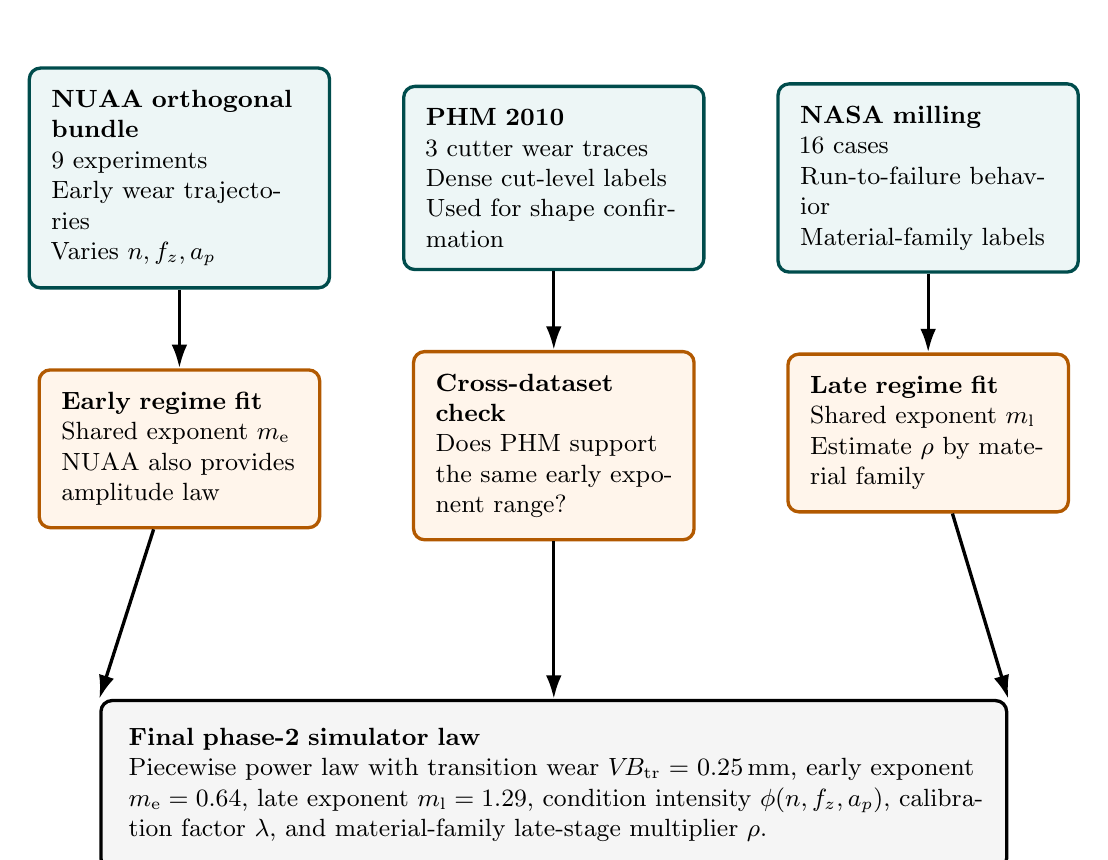
\begin{tikzpicture}[
  font=\small,
  node distance=1.0cm and 0.9cm,
  box/.style={draw=teal!60!black, very thick, rounded corners, fill=teal!7, align=left, inner sep=8pt, text width=3.25cm},
  midbox/.style={draw=orange!70!black, very thick, rounded corners, fill=orange!8, align=left, inner sep=8pt, text width=3.0cm},
  outbox/.style={draw=black, very thick, rounded corners, fill=gray!8, align=left, inner sep=10pt, text width=10.8cm},
  arr/.style={-{Latex[length=3mm,width=2mm]}, very thick}
]
\node[box] (nuaa) {\textbf{NUAA orthogonal bundle}\\9 experiments\\Early wear trajectories\\Varies \(n, f_z, a_p\)};
\node[box, right=of nuaa] (phm) {\textbf{PHM 2010}\\3 cutter wear traces\\Dense cut-level labels\\Used for shape confirmation};
\node[box, right=of phm] (nasa) {\textbf{NASA milling}\\16 cases\\Run-to-failure behavior\\Material-family labels};

\node[midbox, below=of nuaa] (earlyfit) {\textbf{Early regime fit}\\Shared exponent \(m_{\mathrm{e}}\)\\NUAA also provides amplitude law};
\node[midbox, below=of phm] (earlycheck) {\textbf{Cross-dataset check}\\Does PHM support the same early exponent range?};
\node[midbox, below=of nasa] (latefit) {\textbf{Late regime fit}\\Shared exponent \(m_{\mathrm{l}}\)\\Estimate \(\rho\) by material family};

\node[outbox, below=2.0cm of earlycheck] (final) {\textbf{Final phase-2 simulator law}\\
Piecewise power law with transition wear \(\vbtr=\SI{0.25}{mm}\), early exponent \(\earlyexp=\num{0.64}\), late exponent \(\lateexp=\num{1.29}\), condition intensity \(\phii(n,f_z,a_p)\), calibration factor \(\lambda\), and material-family late-stage multiplier \(\rho\).};

\draw[arr] (nuaa) -- (earlyfit);
\draw[arr] (phm) -- (earlycheck);
\draw[arr] (nasa) -- (latefit);
\draw[arr] (earlyfit) -- (final.north west);
\draw[arr] (earlycheck) -- (final);
\draw[arr] (latefit) -- (final.north east);
\end{tikzpicture}
\caption{Native LaTeX diagram of the phase-2 evidence flow. Each dataset contributes to a specific modeling sub-problem rather than to one undifferentiated global fit.}
\label{fig:evidence-flow}
\end{figure}

\subsection{Primary source notes}

The local documentation supports the dataset-role assignment:

\begin{itemize}[leftmargin=1.6em]
\item The Uniwear README states that the NUAA orthogonal bundle contains the \(3 \times 3\) combinations of
feed per tooth \(\{0.045, 0.05, 0.055\}\), spindle speed \(\{1750, 1800, 1850\}\), and corresponding axial depth settings,
making it the natural basis for a parametric early wear law \cite{uniwearrepo}.
\item The same README notes that PHM 2010 contributes cutter wear traces and overlapping signal channels but, in the
local phase-2 use case, the wear files are primarily exploited for wear labels rather than for an explicit parameter-law refit \cite{uniwearrepo}.
\item The NASA documentation identifies the fixed cutting speed of \SI{200}{m/min} (\SI{826}{rpm}),
two depths of cut (\SI{0.75}{mm}, \SI{1.5}{mm}), two feed values (\SI{0.25}{mm/rev}, \SI{0.5}{mm/rev}),
and two material families (cast iron and steel), making it the natural source for late-stage and material-family interpretation \cite{nasa_doc}.
\end{itemize}

\section{Data Preparation and Exploratory Framing}

\subsection{NUAA preprocessing}

The function \code{load\_nuaa\_run\_level()} reads the high-resolution orthogonal bundle and aggregates the raw
timeseries to a run-level table using the latest timestamp and maximum wear in each grouped run. The grouping
variables are \code{experiment\_tag} and \code{experiment\_csv\_n}. The preprocessing then computes:

\begin{itemize}[leftmargin=1.6em]
\item \(t\) in minutes from the original timestamp in seconds,
\item relative time within each experiment,
\item initial wear per experiment,
\item wear increment \(\Delta \vb = \vb - \vb_0\).
\end{itemize}

This choice is conceptually important. The phase-2 model does not predict raw cumulative wear from zero in a
vacuum. It predicts \emph{growth beyond the observed initial condition}. That is why initial wear is carried explicitly
through the later simulator equations.

\subsection{PHM 2010 preprocessing}

The function \code{load\_phm\_cut\_level()} reads the wear tables for cutters \code{c1}, \code{c4}, and \code{c6}.
For each cut, flank wear is defined as the average of the three flute measurements, converted from micrometers to
millimeters. The time-like variable here is not physical minute count but \emph{relative cut index}. That is one reason
PHM 2010 is used in phase-2 to validate wear shape rather than to calibrate absolute minute-based life constants.

\subsection{NASA preprocessing}

The function \code{load\_nasa\_case\_level()} loads case-level flank wear values from
\path{data/nasa_milling/csv/metadata.csv}. Cases are sorted by time, converted to relative time within each case,
and tagged by material family:

\[
\text{material } 1 \mapsto \text{cast\_iron}, \qquad
\text{material } 2 \mapsto \text{steel}.
\]

The NASA documentation confirms that wear measurements were taken at irregular intervals and that not every run
has an associated flank wear observation \cite{nasa_doc}. This irregularity is compatible with the phase-2 estimation
approach because the shared-exponent fit uses the observed pairs \((t, \vb)\) directly rather than assuming uniform
sampling.

\subsection{Exploratory implications}

Even before fitting the final simulator, three exploratory observations are visible:

\begin{enumerate}[leftmargin=1.8em]
\item NUAA does reach wear near and slightly above the chosen transition wear of \SI{0.25}{mm}, but only over a narrow
range. It is best suited to early-stage trend identification, not strong late-stage inference.
\item PHM 2010 provides long wear histories in cut index, supporting the idea that the early regime is not purely linear.
\item NASA reaches far beyond the transition wear and into obvious run-to-failure territory, which makes it essential for
estimating an accelerated terminal regime.
\end{enumerate}

\section{Modeling Strategy}

\subsection{Shared-exponent power law for regime identification}

For each dataset role, phase-2 begins with the same model family:

\begin{equation}
\Delta \vb_g(t) = a_g \, t^m,
\label{eq:group-power}
\end{equation}

where \(g\) indexes an experiment or case, \(a_g\) is a group-specific amplitude, and \(m\) is a shared exponent.
This structure is fitted by nonlinear least squares in \code{fit\_common\_power()}, with one exponent shared across
all groups in the same dataset slice.

The reason for this shared-exponent structure is methodological discipline. If every experiment received its own
exponent, the phase-2 pipeline would lose the ability to claim an interpretable common regime. By forcing a common
\(m\), the fit asks a sharper question: \emph{is there evidence that multiple trajectories share one regime shape, with
variation absorbed mainly through amplitude?}

\subsection{Candidate model check on NUAA}

NUAA is the main early-regime training source, so the code compares two model families:

\begin{itemize}[leftmargin=1.6em]
\item linear in time: \(m = 1\),
\item power in time: \(m\) estimated from data.
\end{itemize}

The generated output \path{phase -2/outputs/nuaa_candidate_models.csv} reports:

\begin{table}[H]
\centering
\caption{NUAA candidate model comparison for the early regime}
\begin{tabular}{lrr}
\toprule
Model & Exponent & RMSE (mm) \\
\midrule
Linear in time & 1.0000 & 0.02676 \\
Power in time & 0.6347 & 0.02113 \\
\bottomrule
\end{tabular}
\end{table}

The power-law model reduces NUAA RMSE by roughly \SI{21}{\percent} relative to the linear-in-time alternative.
This is the first strong empirical reason that phase-2 adopts a sub-linear early regime instead of a classical straight-line
wear approximation.

\subsection{Condition-intensity law from NUAA amplitudes}

Once the early exponent is selected, the code estimates experiment-specific early amplitudes under a \emph{fixed}
exponent and then regresses those amplitudes against normalized process parameters:

\begin{equation}
\log a_g =
\log k_{\mathrm{early}}
 + \alpha_n \log \left(\frac{n}{n_{\mathrm{ref}}}\right)
 + \alpha_f \log \left(\frac{f_z}{f_{z,\mathrm{ref}}}\right)
 + \alpha_a \log \left(\frac{a_p}{a_{p,\mathrm{ref}}}\right).
\label{eq:log-amplitude}
\end{equation}

With the reference settings
\[
n_{\mathrm{ref}} = \SI{1800}{rpm}, \qquad
f_{z,\mathrm{ref}} = \SI{0.05}{mm/tooth}, \qquad
a_{p,\mathrm{ref}} = \SI{3.0}{mm},
\]
the condition-intensity term is
\begin{equation}
\phii(n,f_z,a_p) =
\left(\frac{n}{1800}\right)^{0.35997}
\left(\frac{f_z}{0.05}\right)^{3.95601}
\left(\frac{a_p}{3.0}\right)^{0.68807}.
\label{eq:phi}
\end{equation}

This formulation is central to phase-2. It isolates the early wear \emph{shape} from the process-parameter
\emph{scaling}, which makes the later simulator interpretable and analytically invertible.

\subsection{Late-stage acceleration and material-family ratios}

The NASA dataset is processed differently because its main value lies after the transition region. The code fixes:

\[
\vbtr = \SI{0.25}{mm}, \qquad \earlyexp = 0.64, \qquad \lateexp = 1.29.
\]

For each usable NASA case:

\begin{enumerate}[leftmargin=1.8em]
\item identify the transition time by interpolation at \(\vb = \vbtr\),
\item back out the early amplitude required to reach \(\vbtr\) under the selected early exponent,
\item fit a late-stage amplitude from the post-transition observations under the selected late exponent,
\item define the late-stage multiplier as
\[
\rho = \frac{a_{\mathrm{late}}}{a_{\mathrm{early}}}.
\]
\end{enumerate}

This ratio-based design is prudent. It avoids claiming that the absolute NASA amplitude should replace the absolute
NUAA amplitude law. Instead, NASA contributes what it can support most directly: \emph{how much faster the late
regime evolves relative to the early regime within the same case}.

\subsection{Final phase-2 piecewise equation}

The selected simulator law stored in \path{phase -2/outputs/phase2_model_summary.json} is:

\begin{equation}
\vb(t) = \vb_0 + \lambda \, k_{\mathrm{early}} \, \phii \, t^{\earlyexp},
\qquad \text{for } \vb(t) \le \vbtr,
\label{eq:early-final}
\end{equation}

and

\begin{equation}
\vb(t) = \vbtr + \lambda \, \rho \, k_{\mathrm{early}} \, \phii \, (t-\ttr)^{\lateexp},
\qquad \text{for } \vb(t) > \vbtr,
\label{eq:late-final}
\end{equation}

where \(\lambda\) is a calibration factor for a specific tool-workpiece pair and \(\rho\) is the
late-stage multiplier. The transition time is

\begin{equation}
\ttr =
\left(
\frac{\vbtr - \vb_0}{\lambda \, k_{\mathrm{early}} \, \phii}
\right)^{1/\earlyexp},
\qquad \text{when } \vbtr > \vb_0.
\label{eq:ttr}
\end{equation}

\begin{figure}[H]
\centering
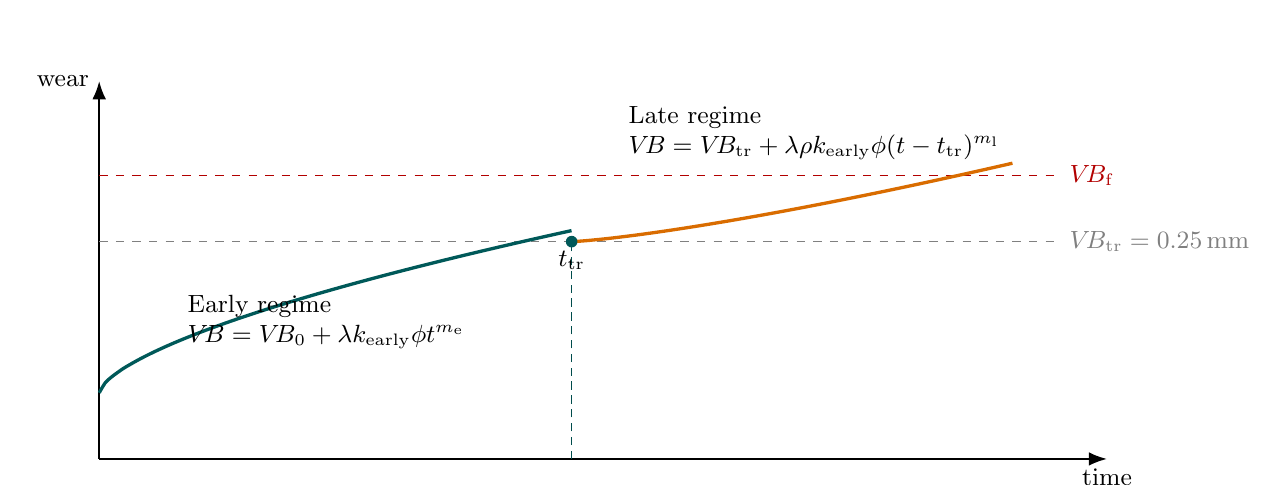
\begin{tikzpicture}[x=2.0cm,y=1.2cm,>=Latex,font=\small]
  \draw[->,thick] (0,0) -- (6.4,0) node[below] {time};
  \draw[->,thick] (0,0) -- (0,4.0) node[left] {wear};
  \draw[dashed,gray] (0,2.3) -- (6.1,2.3) node[right] {\(\vbtr = \SI{0.25}{mm}\)};
  \draw[dashed,red!70!black] (0,3.0) -- (6.1,3.0) node[right] {\(\vbf\)};
  \draw[very thick,teal!70!black,domain=0:3.0,samples=80,smooth] plot (\x,{0.7 + 0.85*pow(\x,0.64)});
  \draw[very thick,orange!85!black,domain=3.0:5.8,samples=80,smooth] plot (\x,{2.3 + 0.22*pow(\x-3.0,1.29)});
  \draw[densely dashed,teal!60!black] (3.0,0) -- (3.0,2.3) node[below,black] {\(\ttr\)};
  \fill[teal!70!black] (3.0,2.3) circle (2.1pt);
  \node[align=left,anchor=west] at (0.5,1.45) {Early regime\\\(\vb = \vb_0 + \lambda k_{\mathrm{early}}\phii t^{\earlyexp}\)};
  \node[align=left,anchor=west] at (3.3,3.45) {Late regime\\\(\vb = \vbtr + \lambda \rho k_{\mathrm{early}}\phii (t-\ttr)^{\lateexp}\)};
\end{tikzpicture}
\caption{Native LaTeX conceptual diagram of the phase-2 piecewise wear law. The early regime is sub-linear; the late regime accelerates after the transition wear.}
\label{fig:piecewise-diagram}
\end{figure}

\subsection{Analytical inversion for threshold life}

The practical strength of the model is that threshold life remains available in closed form.
If the target wear threshold \(\vbf\) lies in the early regime,

\begin{equation}
T_{\mathrm{f}} =
\left(
\frac{\vbf - \vb_0}{\lambda \, k_{\mathrm{early}} \, \phii}
\right)^{1/\earlyexp}.
\label{eq:life-early}
\end{equation}

If \(\vbf > \vbtr\), then

\begin{equation}
T_{\mathrm{f}} = \ttr +
\left(
\frac{\vbf - \vbtr}{\lambda \, \rho \, k_{\mathrm{early}} \, \phii}
\right)^{1/\lateexp}.
\label{eq:life-late}
\end{equation}

That analytic invertibility is a key reason the explicit phase-2 equation remains valuable even though a simple linear
regression outperforms it on one held-out NUAA benchmark, as discussed later.

\subsection{Calibration from one measured point}

The simulator also exposes a direct formula for \(\lambda\) from a measured early-stage wear point
\((t_{\mathrm{obs}}, \vb_{\mathrm{obs}})\):

\begin{equation}
\lambda =
\frac{\vb_{\mathrm{obs}} - \vb_0}
{k_{\mathrm{early}} \, \phii \, t_{\mathrm{obs}}^{\earlyexp}},
\label{eq:lambda}
\end{equation}

provided the observation is in the early regime and exceeds the initial wear.
This is scientifically useful because it separates the shared phase-2 law from specimen-specific absolute scaling.

\section{Main Results}

\subsection{Fitted exponents and selected operating coefficients}

The generated key results support a two-regime interpretation:

\begin{table}[H]
\centering
\caption{Primary fitted exponents and selected coefficients}
\begin{tabularx}{\textwidth}{>{\raggedright\arraybackslash}p{4.0cm}rrX}
\toprule
Quantity & Value & Rounded/selected & Interpretation \\
\midrule
NUAA early exponent & 0.6347 & 0.64 & Sub-linear early wear law under orthogonal milling conditions. \\
PHM early exponent & 0.6471 & 0.64 & Independent confirmation that early milling wear remains near the same exponent range. \\
NASA late exponent & 1.2873 & 1.29 & Accelerated late-stage wear under run-to-failure behavior. \\
\(k_{\mathrm{early}}\) & 0.018581 & 0.018581 & Early wear amplitude at the reference condition. \\
Speed exponent & 0.3600 & 0.3600 & Weakest process exponent among the three fitted NUAA factors. \\
Feed exponent & 3.9560 & 3.9560 & Dominant fitted sensitivity in the early condition law. \\
Depth exponent & 0.6881 & 0.6881 & Clear secondary effect relative to feed. \\
Amplitude \(R^2\) & 0.7679 & 0.7679 & Fraction of log-amplitude variance explained by the normalized NUAA parameter law. \\
\bottomrule
\end{tabularx}
\label{tab:key-results}
\end{table}

Two observations deserve emphasis.

First, the raw exponents from NUAA and PHM are close enough that rounding to a common \(\earlyexp = 0.64\) is
not arbitrary; it is an engineering simplification backed by two distinct early-stage datasets. Second, the feed exponent
is an order of magnitude more influential than the speed exponent within the normalized early-law fit. That does not
prove feed is universally the dominant milling wear driver, but it does show that within the NUAA orthogonal range,
feed changes explain far more amplitude variation than spindle speed changes.

\subsection{Early-regime evidence from NUAA and PHM}

\begin{figure}[H]
\centering
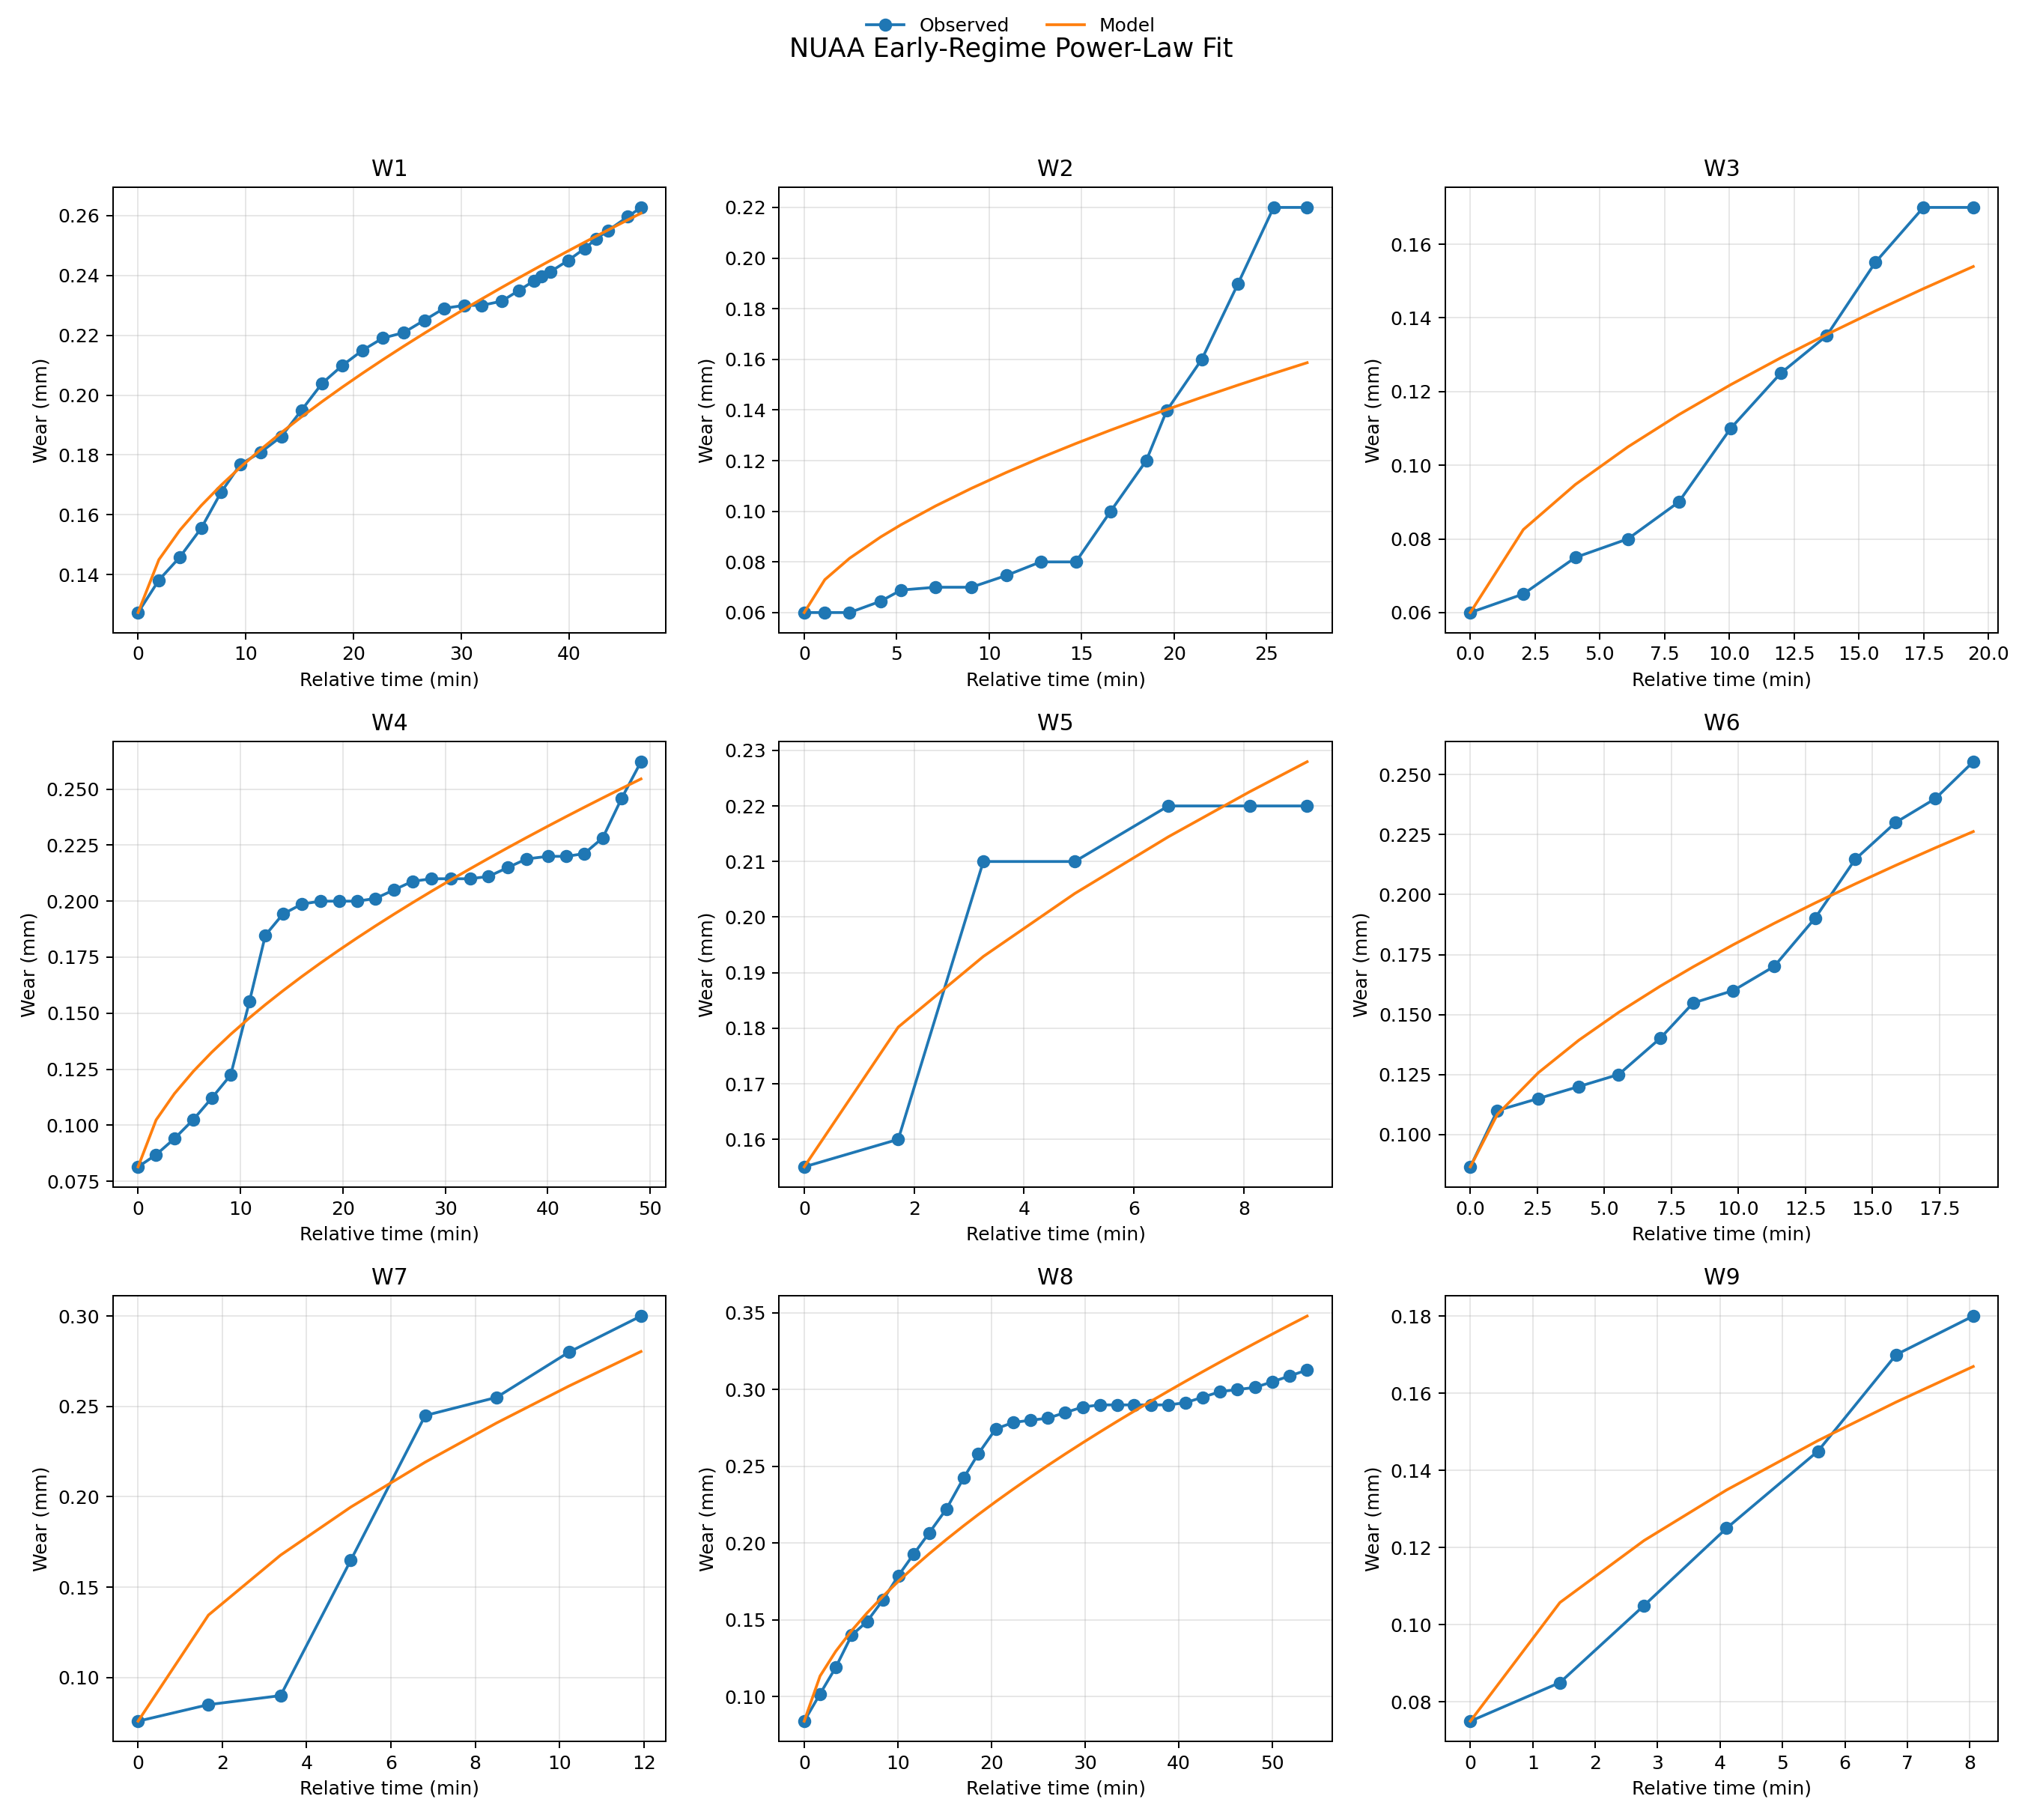
\includegraphics[width=\textwidth,height=0.76\textheight,keepaspectratio]{../plots/nuaa_early_regime_fit.png}
\caption{Observed versus modeled early-regime wear trajectories for the NUAA orthogonal experiments.}
\label{fig:nuaa-fit}
\end{figure}

Figure~\ref{fig:nuaa-fit} shows that the power-law family follows the main curvature of the orthogonal NUAA
experiments without forcing a straight-line increase in wear. Experiments at higher feed and more severe combinations
shift upward primarily through amplitude, which is exactly the structural assumption used later in the parameter law.

\begin{figure}[H]
\centering
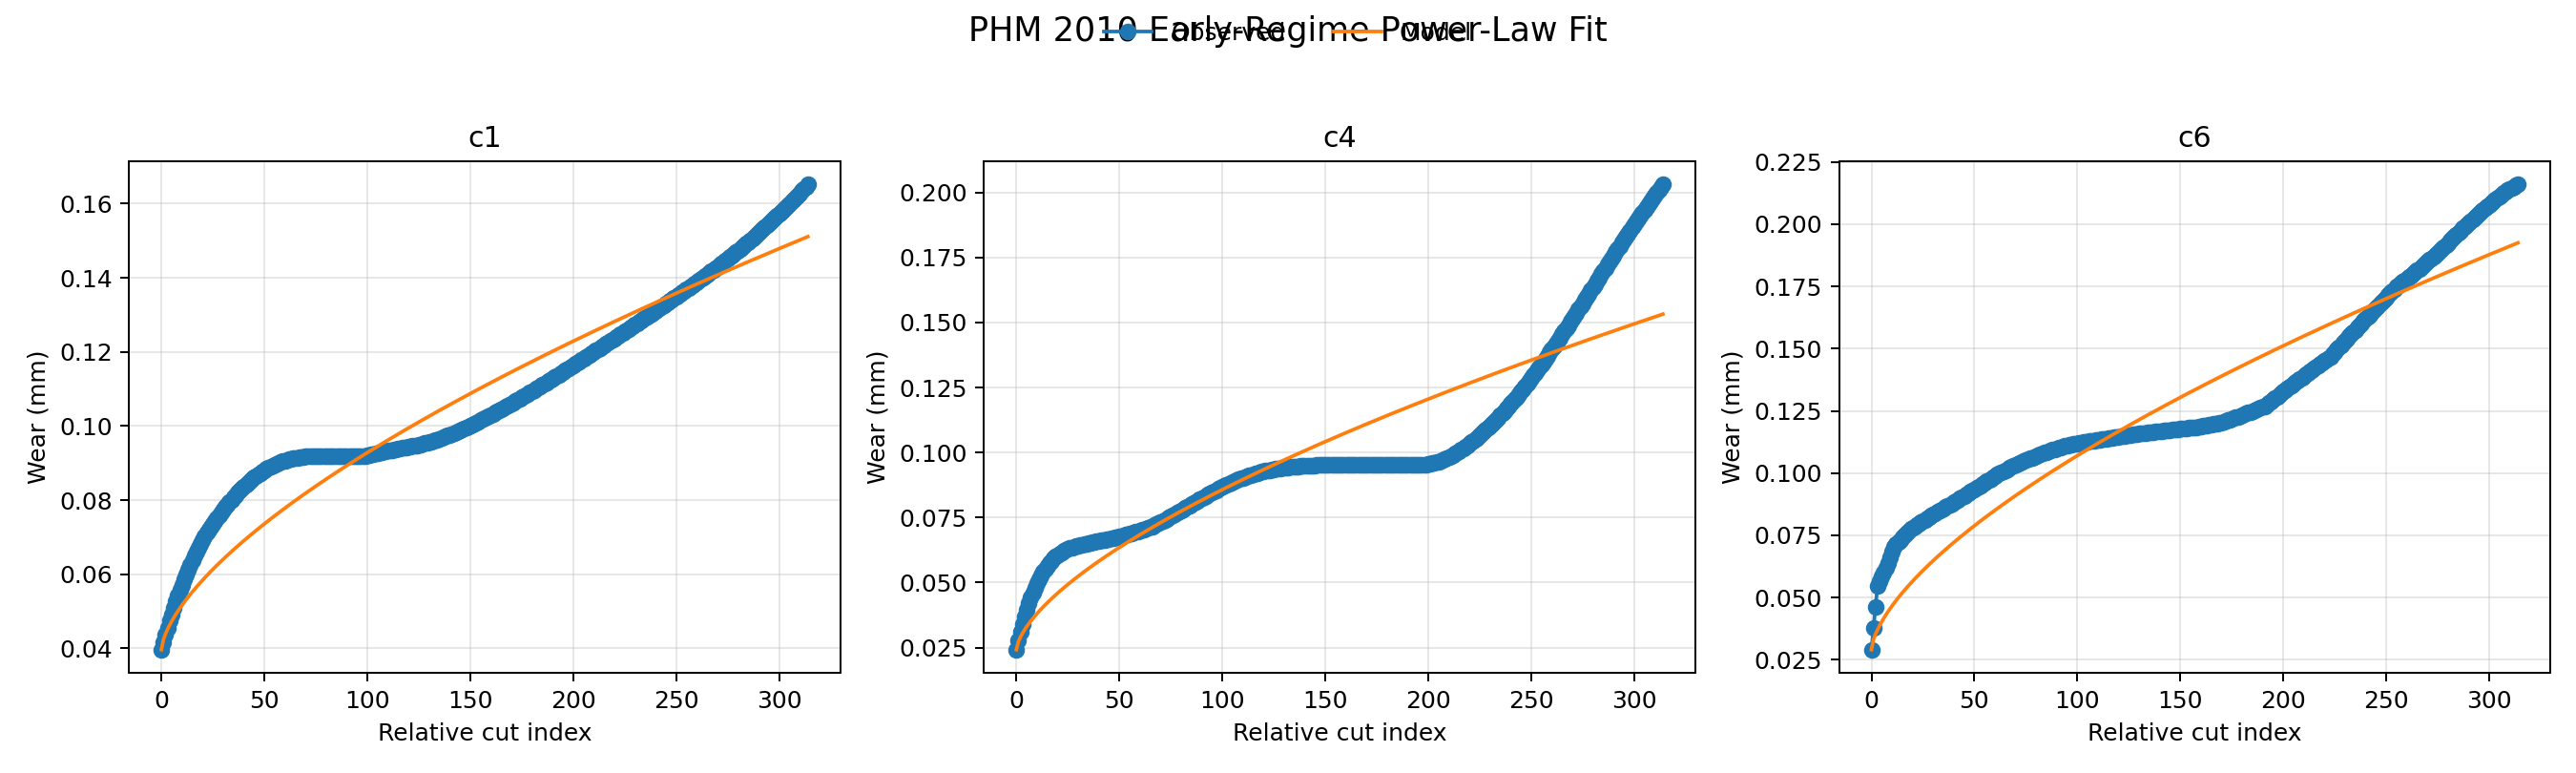
\includegraphics[width=\textwidth,height=0.76\textheight,keepaspectratio]{../plots/phm_early_regime_fit.png}
\caption{Observed versus modeled wear trajectories for the PHM 2010 cutter wear data, used as a cross-dataset check on early-regime shape.}
\label{fig:phm-fit}
\end{figure}

Figure~\ref{fig:phm-fit} is important because it checks whether the early-stage exponent is merely a quirk of the
NUAA bundle. The fitted PHM exponent of \num{0.6471} says it is not. Even though the PHM time axis is cut index rather
than minute count, the early wear curvature remains in the same neighborhood.

\subsection{Late-regime evidence from NASA}

\begin{figure}[H]
\centering
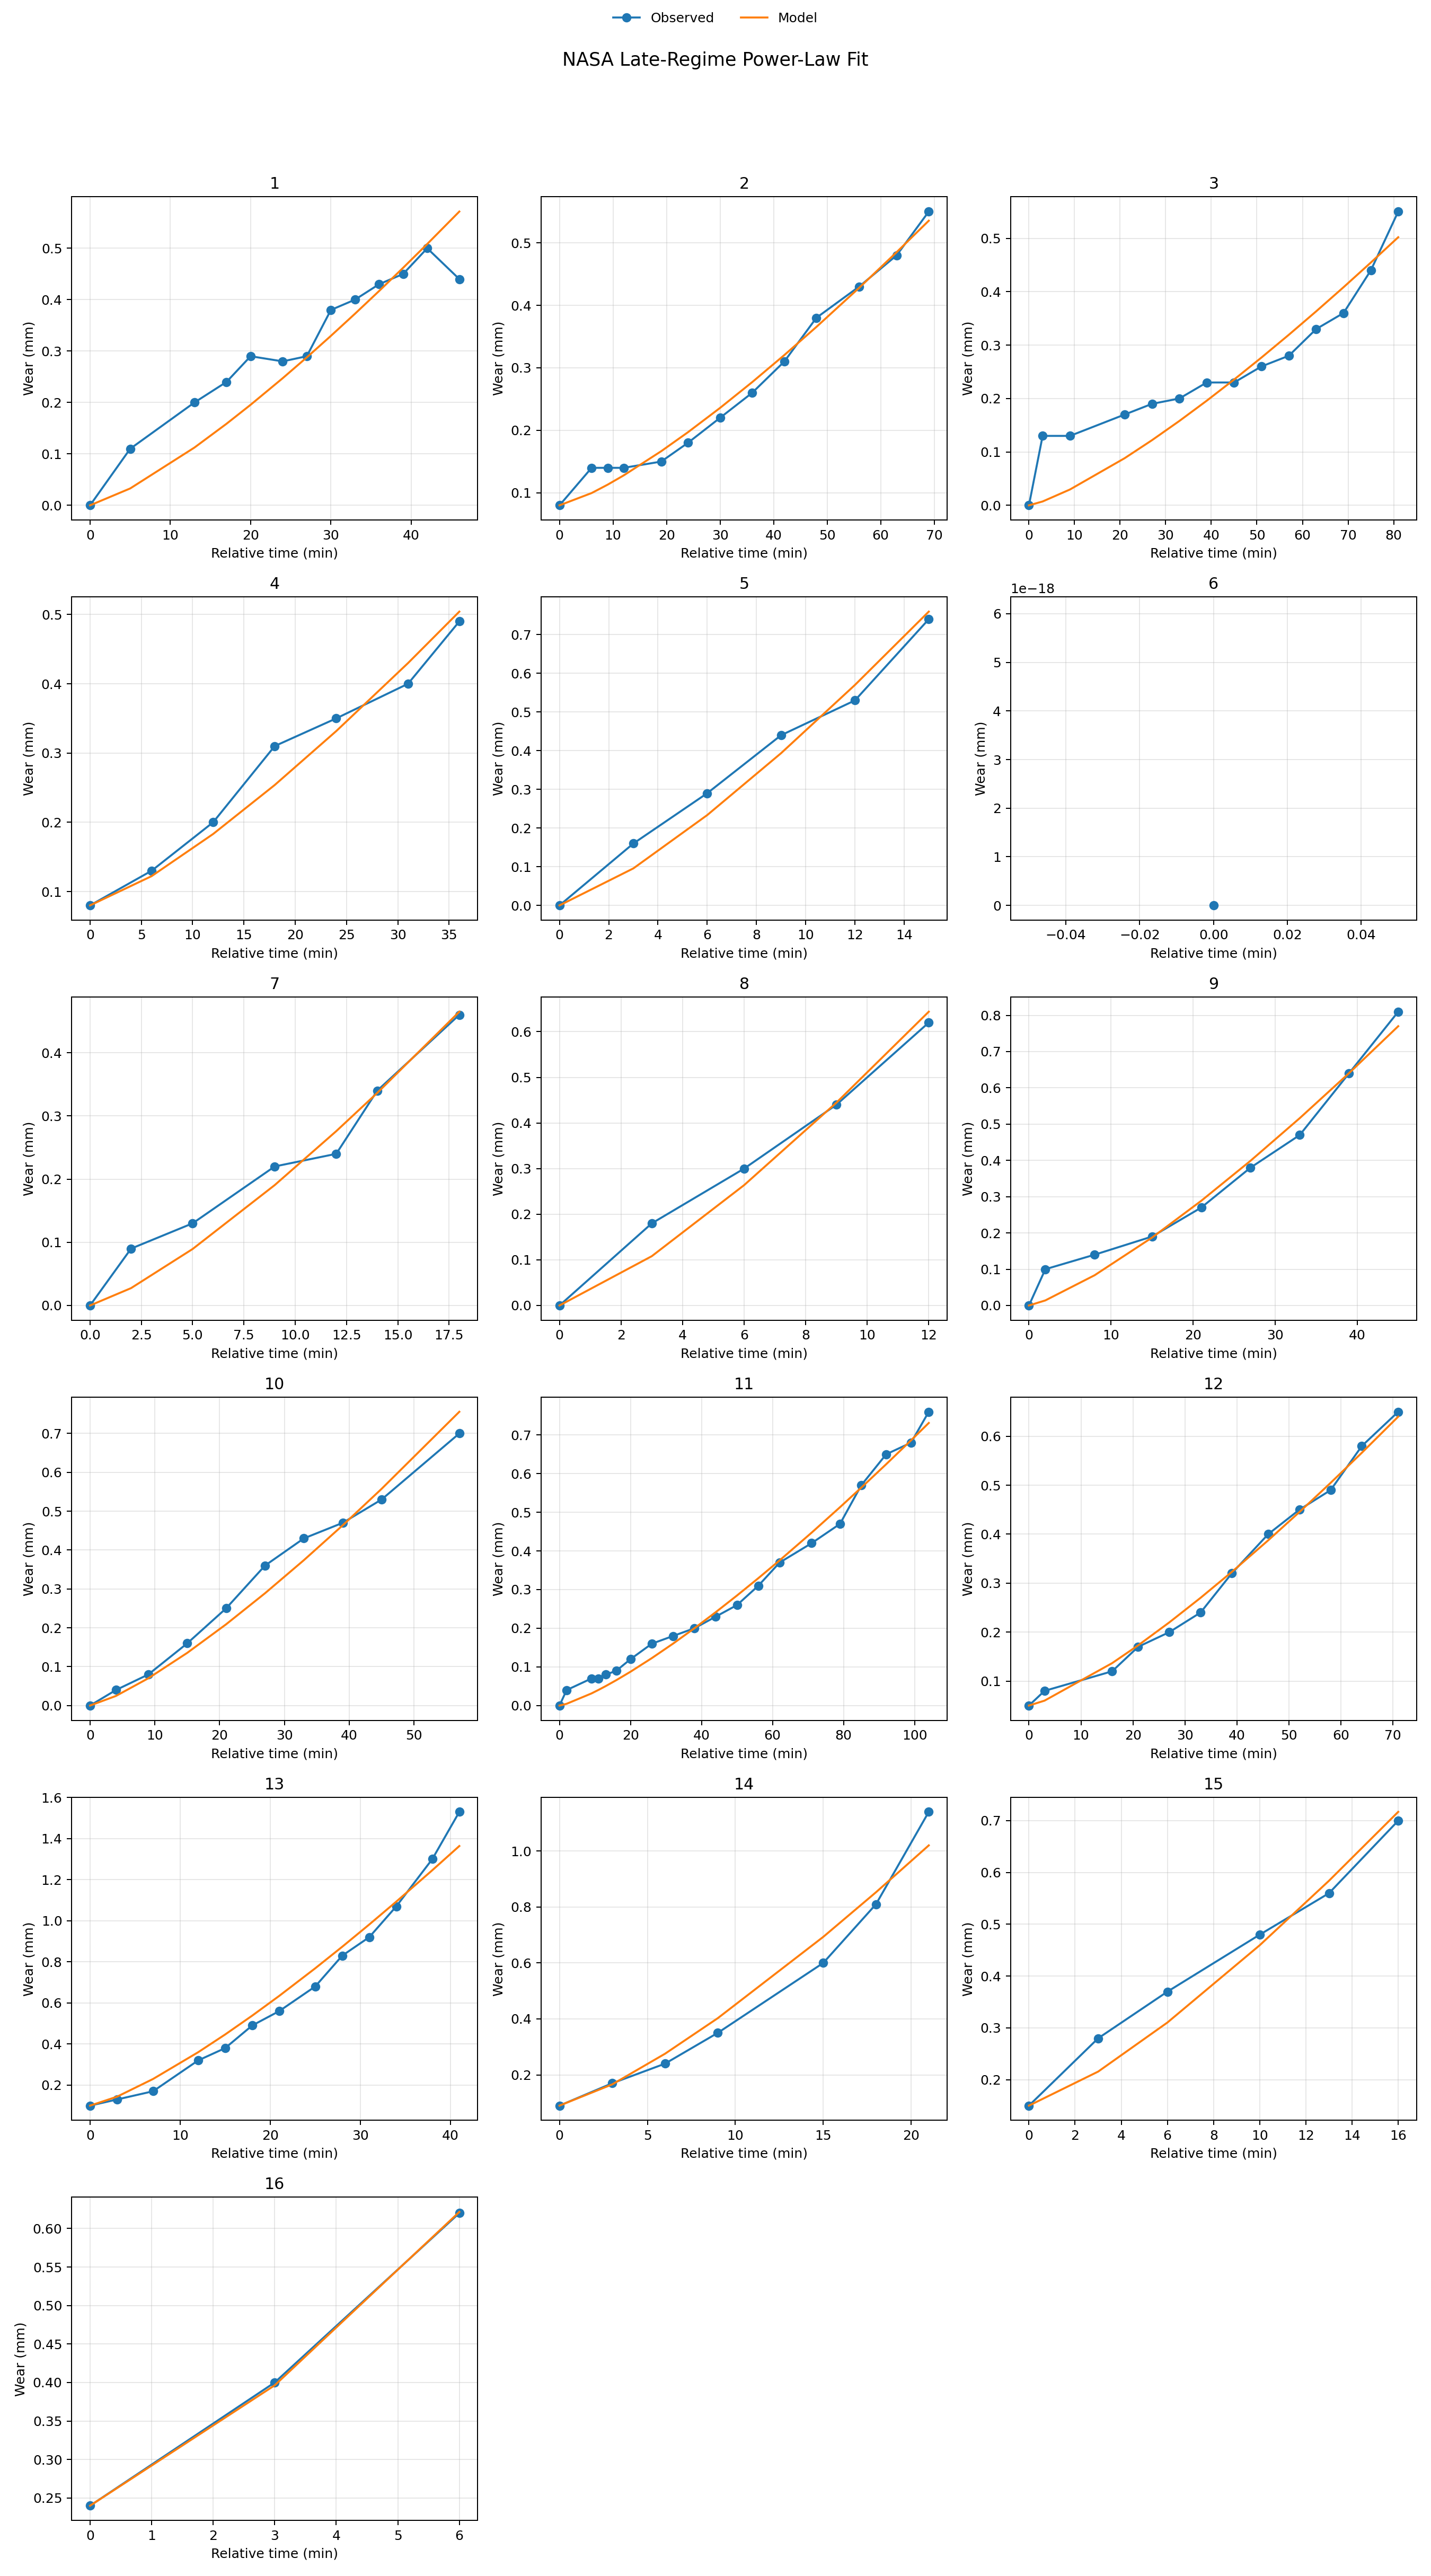
\includegraphics[width=\textwidth,height=0.76\textheight,keepaspectratio]{../plots/nasa_late_regime_fit.png}
\caption{Observed versus modeled NASA late-regime wear trajectories. These cases provide the main evidence for end-of-life acceleration.}
\label{fig:nasa-fit}
\end{figure}

Figure~\ref{fig:nasa-fit} provides the empirical justification for abandoning a single-regime law.
The later portions of the NASA cases are not adequately described by simply extending the early sub-linear regime.
The fitted shared late exponent of \num{1.2873} supports an accelerating tail.

\subsection{Condition-law fit quality}

\begin{figure}[H]
\centering
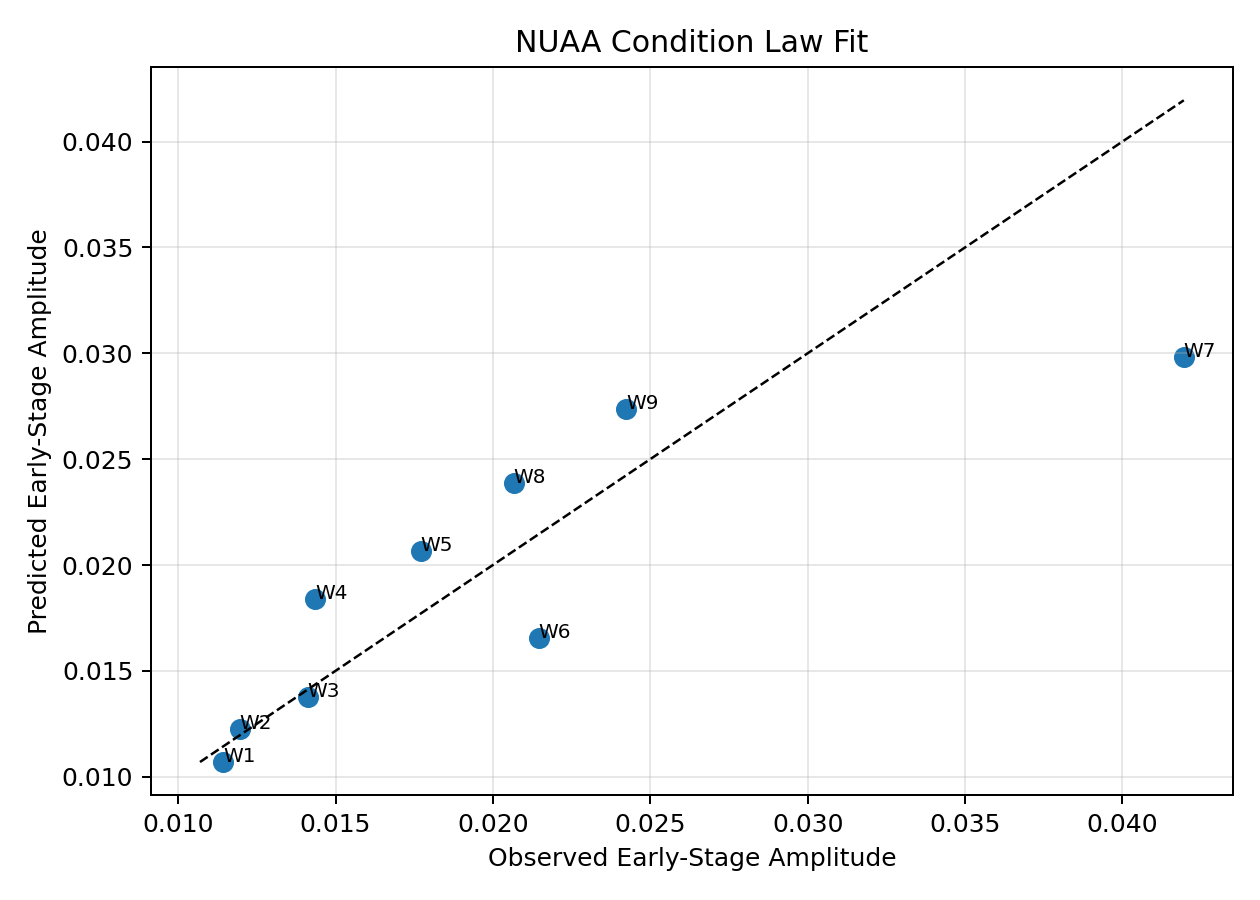
\includegraphics[width=0.78\textwidth]{../plots/nuaa_condition_law_fit.png}
\caption{Observed versus predicted early-stage amplitudes under the NUAA parameter law.}
\label{fig:condition-fit}
\end{figure}

The condition-law fit in Figure~\ref{fig:condition-fit} is not perfect, but it is strong enough to justify a compact
three-parameter early amplitude law. The reported amplitude \(R^2 = \num{0.7679}\) indicates that the normalized
log-linear parameter relation captures most, though not all, of the amplitude variation across the nine orthogonal experiments.

\subsection{Bootstrap stability}

The report builder already generated bootstrap exponent distributions for the three dataset roles. The summary statistics are:

\begin{table}[H]
\centering
\caption{Bootstrap summaries for the shared-exponent fits}
\begin{tabular}{lrrrrr}
\toprule
Dataset role & Mean & Std. dev. & 2.5\% & Median & 97.5\% \\
\midrule
NUAA early & 0.7160 & 0.1968 & 0.5192 & 0.6450 & 1.2731 \\
PHM early & 0.6521 & 0.0519 & 0.5917 & 0.6471 & 0.7949 \\
NASA late & 1.2706 & 0.1214 & 1.0216 & 1.2752 & 1.4806 \\
\bottomrule
\end{tabular}
\label{tab:bootstrap}
\end{table}

\begin{figure}[H]
\centering
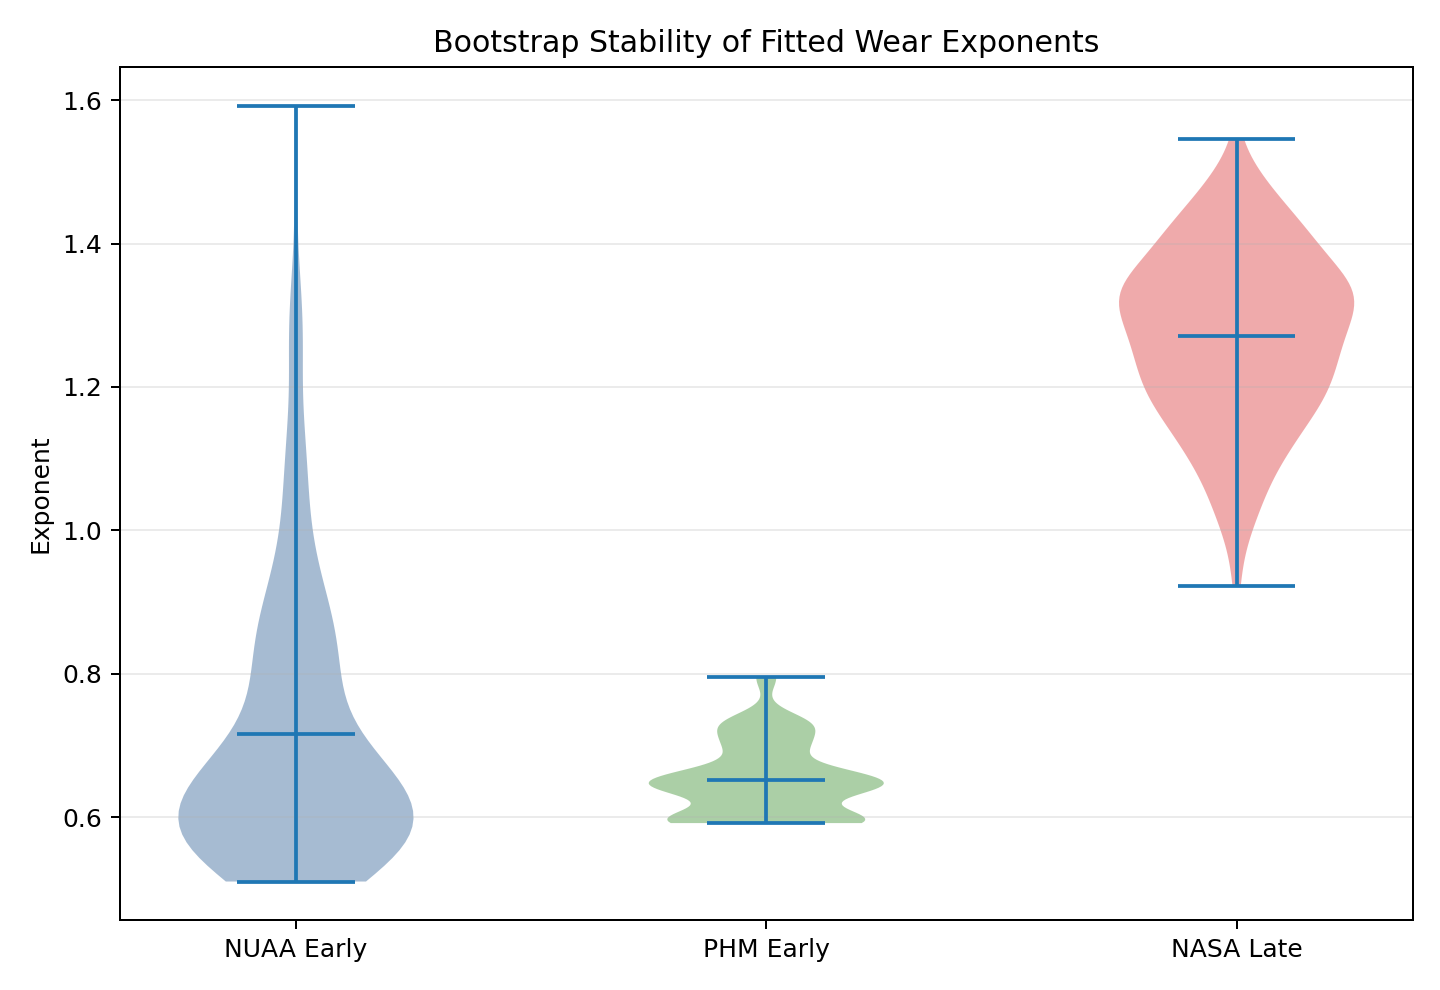
\includegraphics[width=0.82\textwidth]{../plots/bootstrap_exponent_stability.png}
\caption{Bootstrap stability of the fitted exponents across the three dataset roles.}
\label{fig:bootstrap}
\end{figure}

The bootstrap distributions make the research interpretation more nuanced.
PHM provides the tightest support for the early exponent, centered almost exactly at the selected value of \num{0.64}.
NASA supports a clearly larger late exponent. NUAA is visibly broader. That broader distribution is not fatal, but it does
warn against over-claiming numerical precision from only nine orthogonal experiments. In phase-2, the wide NUAA tail is
counterbalanced by the PHM confirmation of the early-regime range.

\subsection{Material-family late-stage ratios}

The NASA-derived material-family summaries are:

\begin{table}[H]
\centering
\caption{Late-stage multiplier summaries estimated from NASA case ratios}
\begin{tabular}{lrrrr}
\toprule
Material family & Count & Mean ratio & Median ratio & Suggested \(\rho\) \\
\midrule
Cast iron & 8 & 0.1568 & 0.1488 & 0.1488 \\
Steel & 7 & 0.5062 & 0.3994 & 0.3994 \\
Generic default & -- & -- & -- & 0.2500 \\
\bottomrule
\end{tabular}
\label{tab:late-ratios}
\end{table}

The interquartile ranges from the case table are approximately \([0.1352, 0.1846]\) for cast iron and
\([0.2997, 0.4831]\) for steel. This means the steel late-stage ratio is not only higher in median but also substantially
more variable.

\begin{figure}[H]
\centering
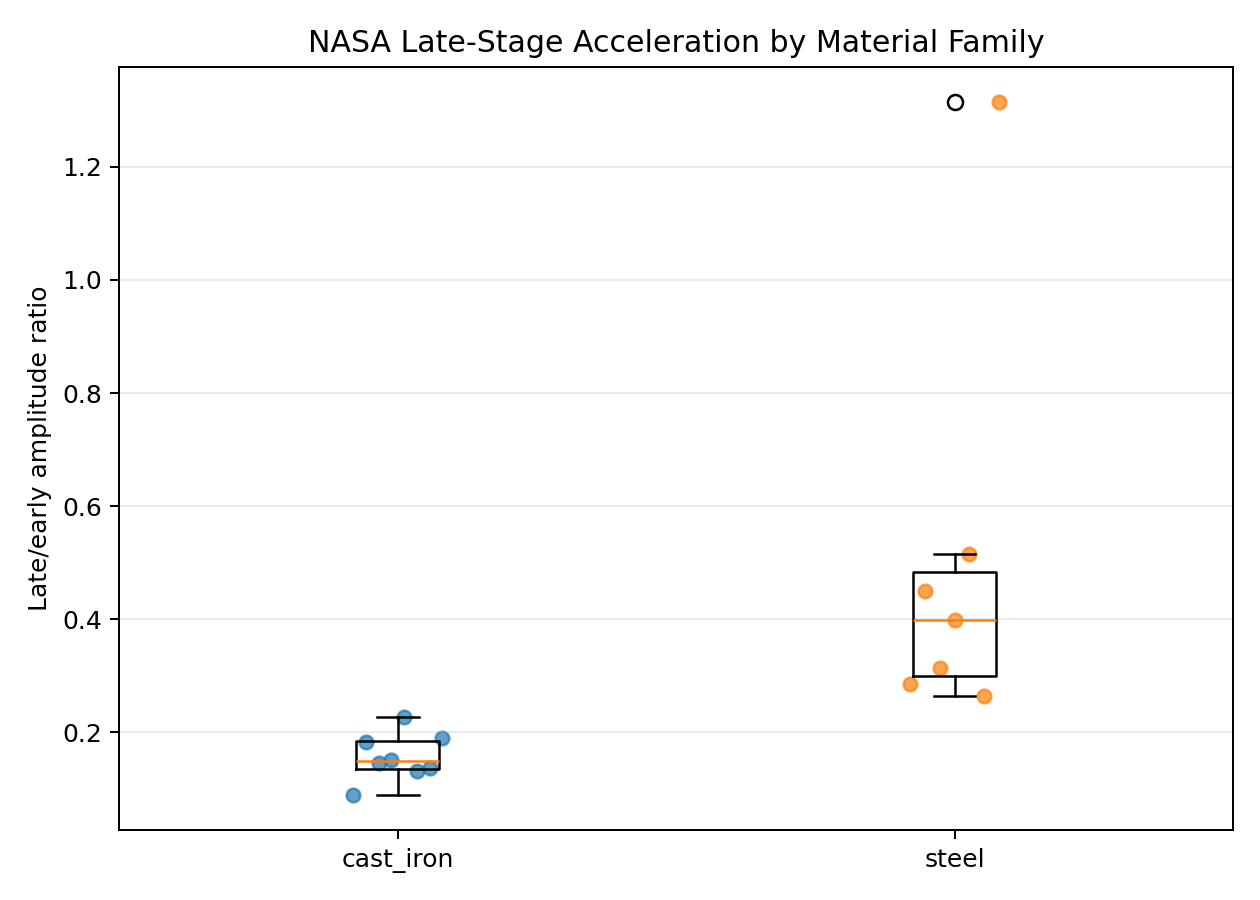
\includegraphics[width=0.72\textwidth]{../plots/nasa_late_stage_materials.png}
\caption{Material-family distribution of late-to-early amplitude ratios in the NASA cases.}
\label{fig:materials}
\end{figure}

One subtle but important detail is that the \emph{generic} late-stage factor of \num{0.25} in the final JSON is not the
median of a pooled NASA fit. It is a neutral engineering default retained by the code and then supplemented with the
data-derived medians for cast iron and steel. That makes the material-specific values research-backed and the generic
value pragmatic rather than strongly evidential.

\section{Validation Against Alternative Predictors}

\subsection{Leave-one-experiment-out benchmark on NUAA}

The phase-2 report builder benchmarks the explicit equation against three machine-learning baselines under
leave-one-experiment-out cross-validation on NUAA:

\begin{table}[H]
\centering
\caption{NUAA leave-one-experiment-out benchmark}
\begin{tabular}{lrrr}
\toprule
Model & RMSE (mm) & MAE (mm) & \(R^2\) \\
\midrule
Linear Regression & 0.03358 & 0.02625 & 0.7742 \\
Random Forest & 0.03763 & 0.02798 & 0.7164 \\
Equation & 0.04371 & 0.03157 & 0.6174 \\
XGBoost & 0.04499 & 0.03680 & 0.5946 \\
\bottomrule
\end{tabular}
\label{tab:benchmark}
\end{table}

\begin{figure}[H]
\centering
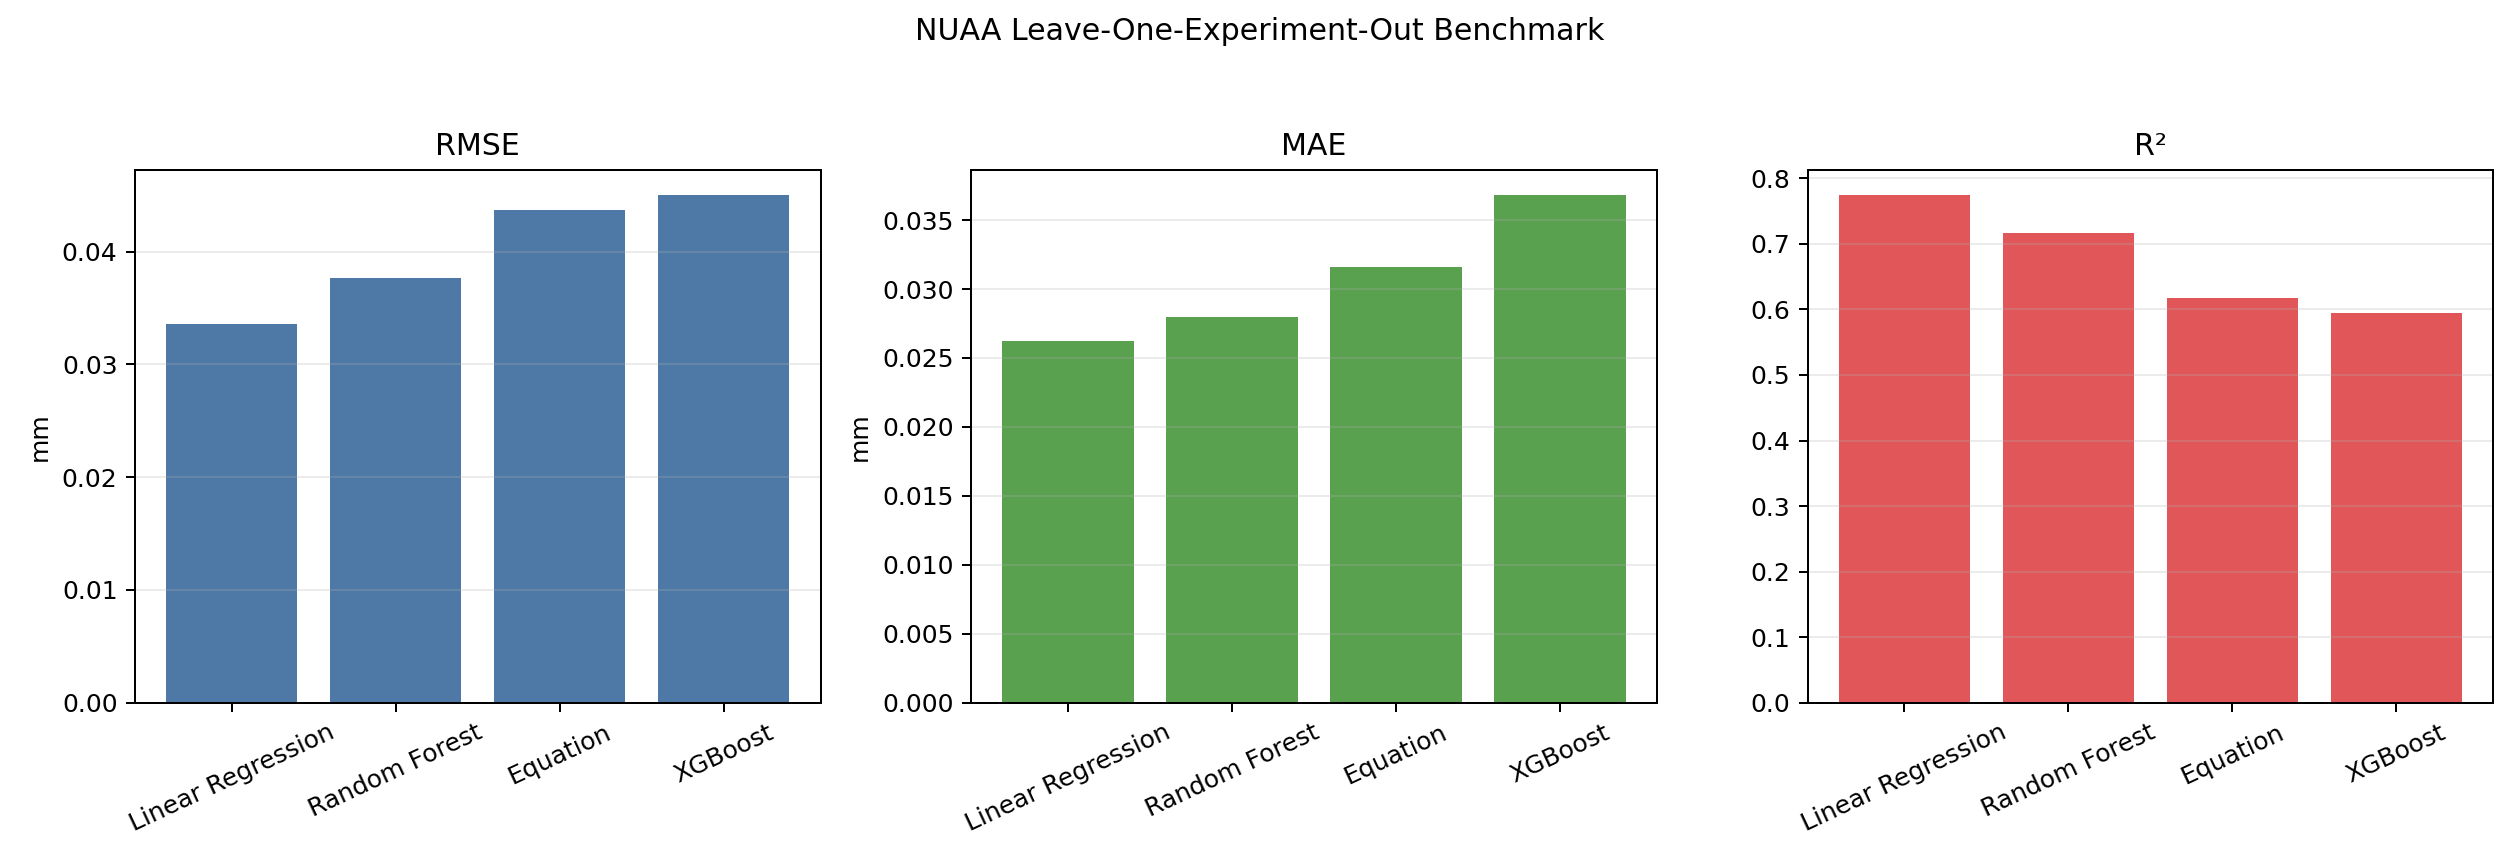
\includegraphics[width=0.88\textwidth]{../plots/nuaa_loeo_benchmark.png}
\caption{NUAA leave-one-experiment-out benchmark across the explicit equation and machine-learning baselines.}
\label{fig:benchmark}
\end{figure}

\subsection{Interpretation of the benchmark}

From a pure point-prediction perspective, the explicit equation is not the best held-out regressor on NUAA.
Relative to linear regression, the equation has an RMSE disadvantage of approximately \SI{0.0101}{mm}, an MAE
disadvantage of \SI{0.0053}{mm}, and a lower \(R^2\) by about \num{0.157}.

That finding should not be hidden. It is part of the honest research record. But it also does not invalidate the phase-2
equation, because the research goal is broader than pointwise curve fitting. The explicit equation retains three properties
that the benchmarked ML models do not provide directly:

\begin{itemize}[leftmargin=1.6em]
\item closed-form inversion to target life, as in Equations~\ref{eq:life-early} and \ref{eq:life-late},
\item direct exposure of machining parameters in the governing law,
\item explicit, interpretable separation between global regime structure and specimen-specific calibration.
\end{itemize}

In other words, the equation loses to linear regression as a held-out wear interpolator on NUAA, but it wins as a
\emph{simulator model}.

\begin{figure}[H]
\centering
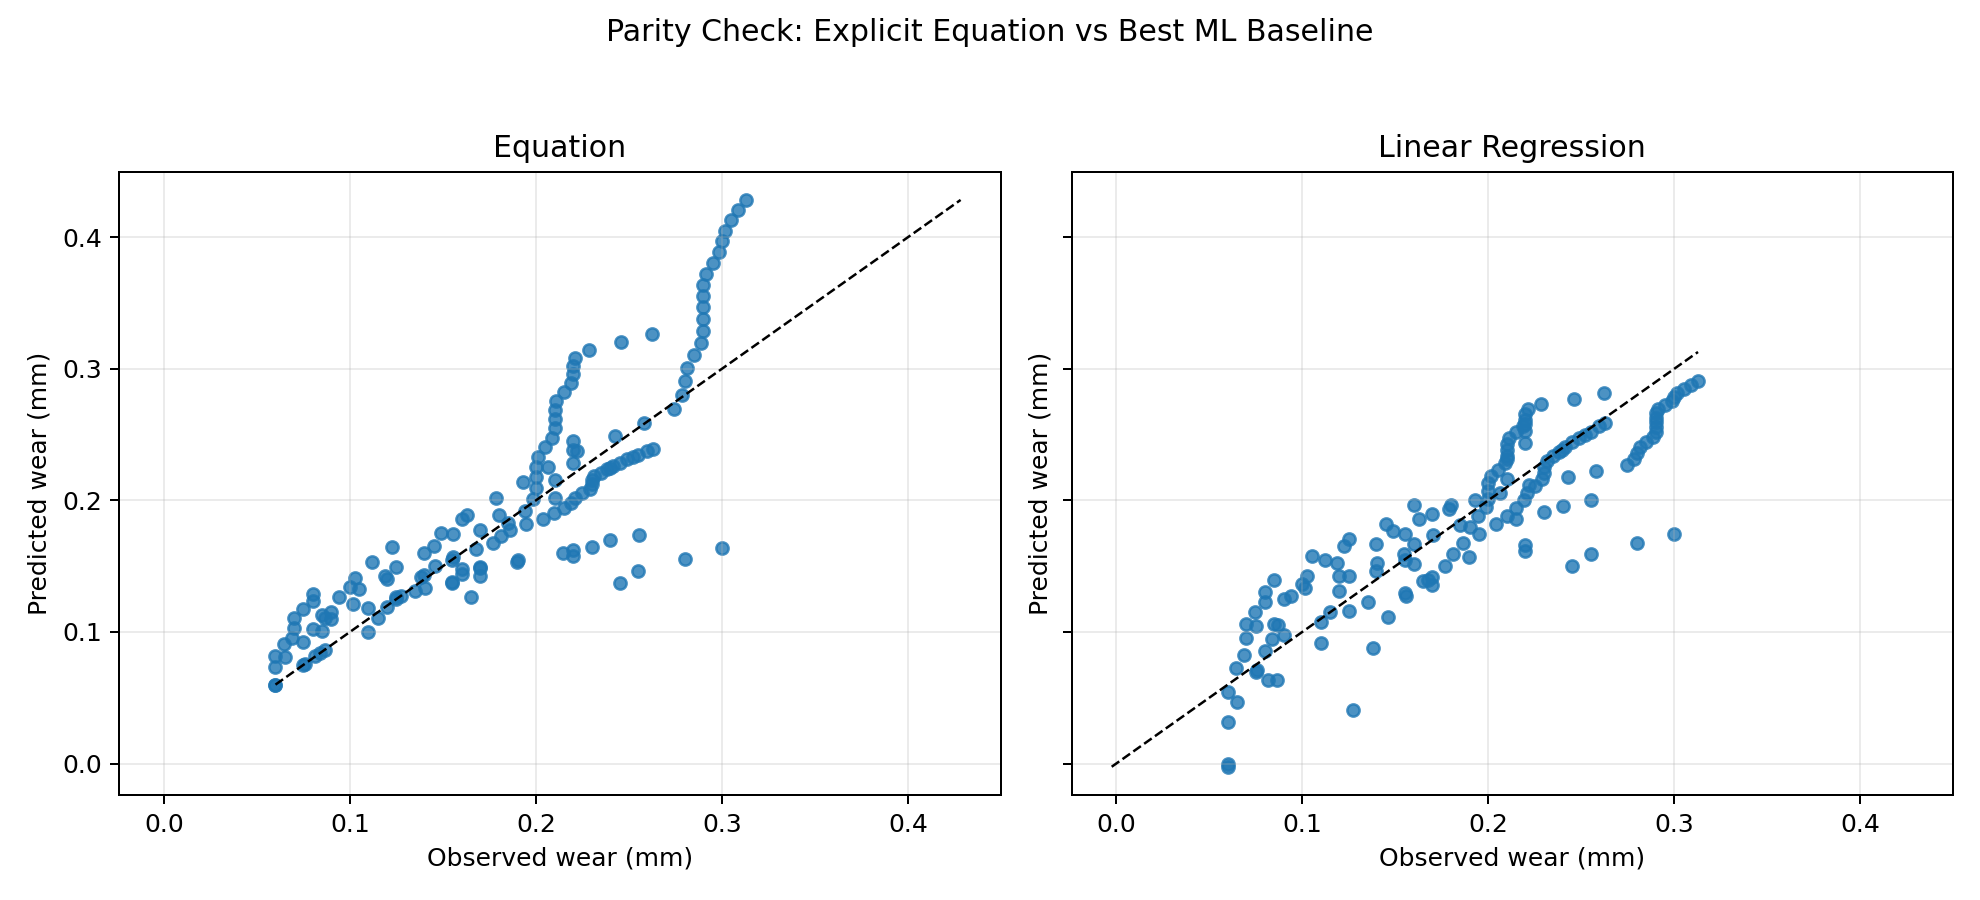
\includegraphics[width=0.84\textwidth]{../plots/nuaa_parity_equation_vs_linear.png}
\caption{Parity comparison of the explicit equation and the strongest simple baseline.}
\label{fig:parity}
\end{figure}

Figure~\ref{fig:parity} reinforces that distinction. Linear regression tracks the held-out NUAA values more tightly,
but the explicit equation remains structurally coherent and physically interpretable rather than purely statistical.

\section{Simulator Behavior and Engineering Interpretation}

\subsection{Baseline scenario}

Using \path{phase -2/tool_life_simulator.py} with the stored coefficients, the following baseline scenario
can be evaluated:

\[
\begin{aligned}
n &= \SI{1800}{rpm}, & f_z &= \SI{0.05}{mm/tooth}, & a_p &= \SI{3.0}{mm}, \\
\vb_0 &= \SI{0.05}{mm}, & \vbf &= \SI{0.30}{mm}, & \lambda &= 1.
\end{aligned}
\]

The corresponding predicted lives are:

\begin{table}[H]
\centering
\caption{Illustrative simulator outputs around the phase-2 baseline}
\begin{tabularx}{\textwidth}{>{\raggedright\arraybackslash}p{6.2cm}rrr}
\toprule
Scenario & \(\phii\) & Life to \SI{0.30}{mm} (min) & Wear at \SI{45}{min} (mm) \\
\midrule
Baseline, generic & 1.0000 & 47.2768 & 0.2781 \\
Baseline, cast iron & 1.0000 & 50.4007 & 0.2667 \\
Baseline, steel & 1.0000 & 45.3554 & 0.2948 \\
Low load (\SI{1750}{rpm}, \SI{0.045}{mm/tooth}, \SI{2.5}{mm}) & 0.5756 & 106.7975 & 0.1722 \\
High load (\SI{1850}{rpm}, \SI{0.055}{mm/tooth}, \SI{3.5}{mm}) & 1.6372 & 23.2686 & 0.7596 \\
\bottomrule
\end{tabularx}
\label{tab:sim-scenarios}
\end{table}

The low-load to high-load life swing is roughly a factor of \num{4.59}. That wide ratio is consistent with the very strong
fitted feed exponent and the moderate depth effect. It is also why the simulator is useful despite the compactness of the
equation: small moves in the operating point can create large moves in predicted life.

\begin{figure}[H]
\centering
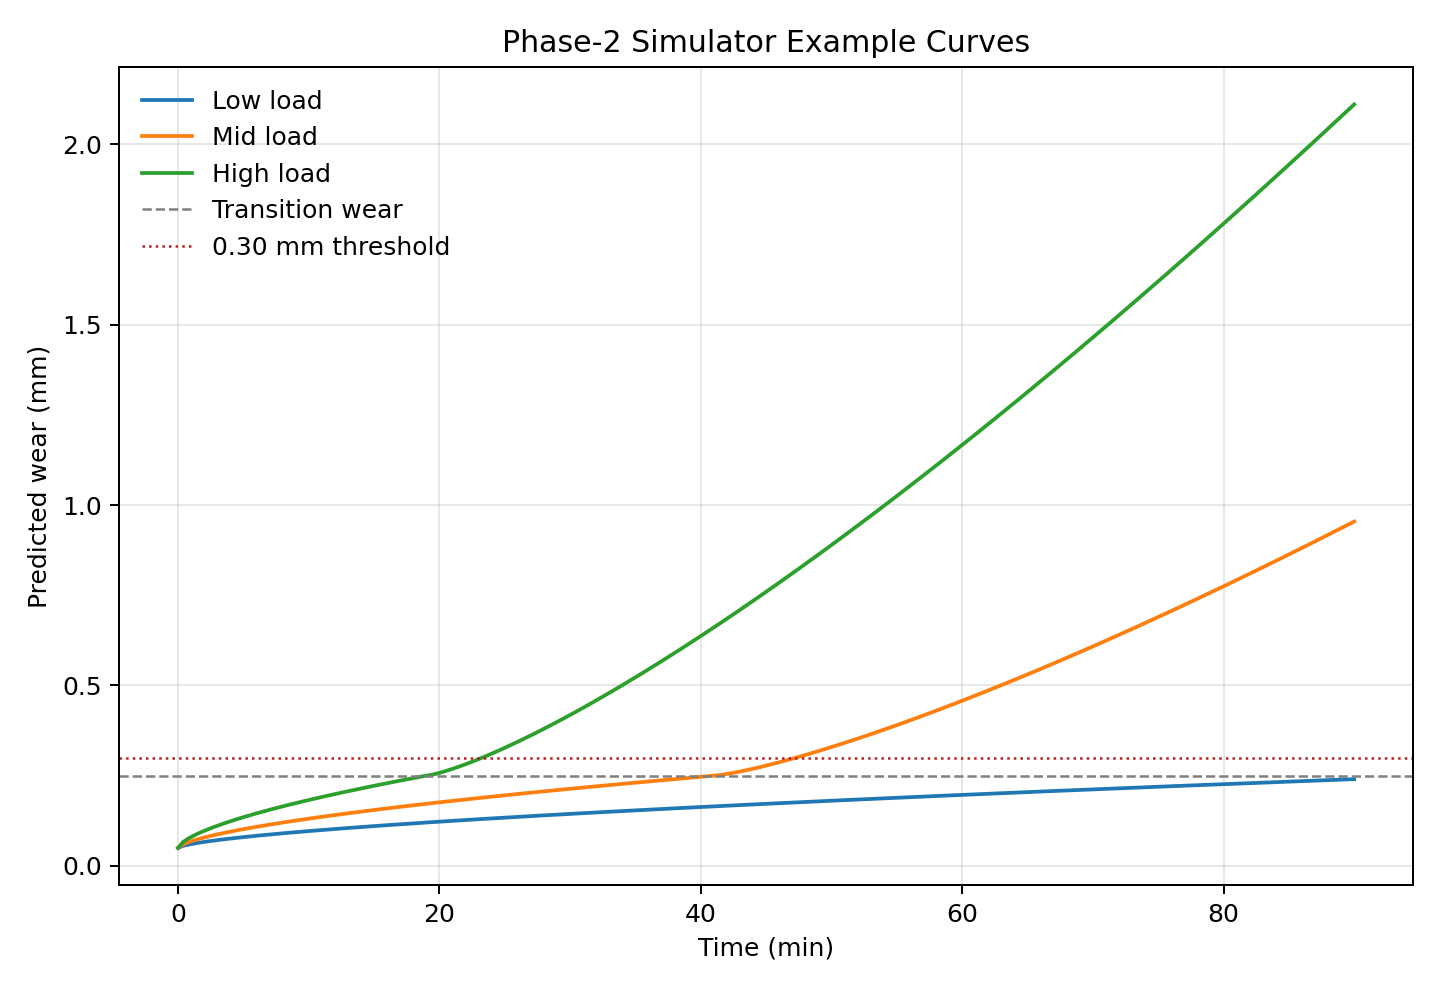
\includegraphics[width=0.82\textwidth]{../plots/simulation_example_curves.png}
\caption{Example simulated wear trajectories under low, medium, and high load conditions.}
\label{fig:sim-curves}
\end{figure}

\subsection{Sensitivity around the reference condition}

\begin{figure}[H]
\centering
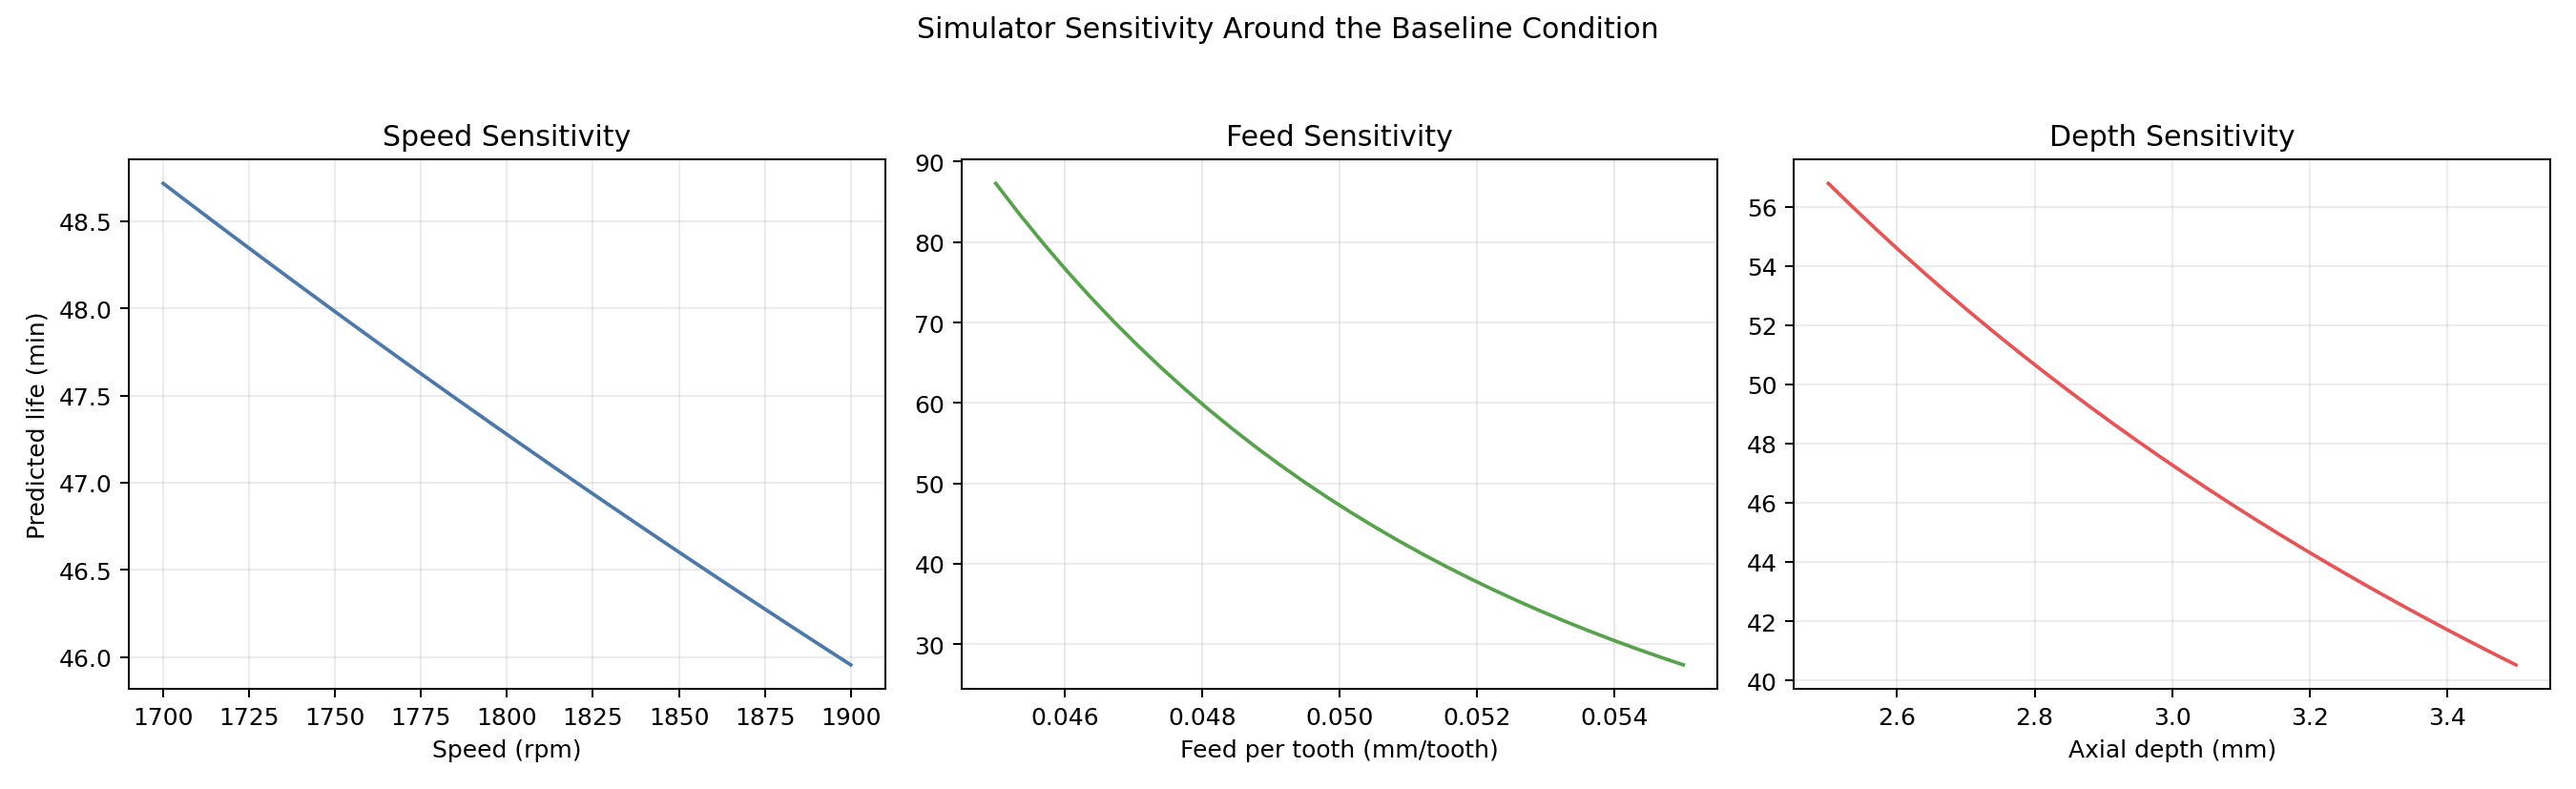
\includegraphics[width=\textwidth]{../plots/life_sensitivity_curves.png}
\caption{Predicted life sensitivity around the reference condition.}
\label{fig:sensitivity}
\end{figure}

Figure~\ref{fig:sensitivity} is especially useful for interpretation.
The speed curve is comparatively shallow, which is consistent with the fitted speed exponent of only \num{0.3600}.
The feed curve is steepest, consistent with the fitted exponent of \num{3.9560}. Depth matters, but less strongly than feed.
This does not prove a universal ranking for all milling systems; it documents the ranking supported by the local phase-2 data.

\subsection{Calibration workflow}

The simulator is most defensible when \(\lambda\) is treated as a calibration quantity rather than silently fixed to one.
The phase-2 codebase already includes the formula to estimate \(\lambda\) from one observed early wear point, and the
research frontend created in the workspace exposes this interaction in the browser.

\begin{figure}[H]
\centering
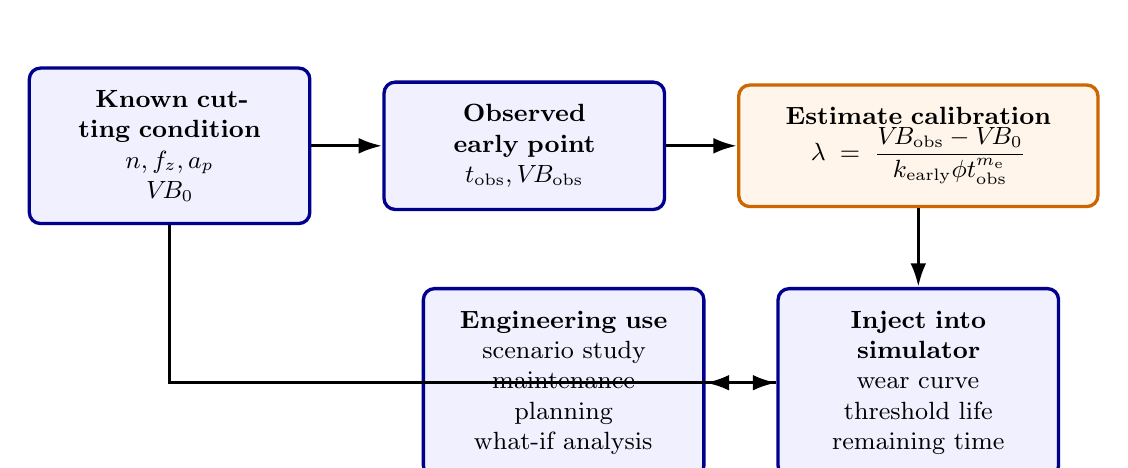
\begin{tikzpicture}[
  font=\small,
  node distance=1.0cm and 0.9cm,
  box/.style={draw=blue!55!black, very thick, rounded corners, fill=blue!6, align=center, inner sep=8pt, text width=3.0cm},
  formula/.style={draw=orange!80!black, very thick, rounded corners, fill=orange!8, align=center, inner sep=8pt, text width=4.0cm},
  arr/.style={-{Latex[length=3mm,width=2mm]}, very thick}
]
\node[box] (inputs) {\textbf{Known cutting condition}\\\(n, f_z, a_p\)\\\(\vb_0\)};
\node[box, right=of inputs] (obs) {\textbf{Observed early point}\\\(t_{\mathrm{obs}}, \vb_{\mathrm{obs}}\)};
\node[formula, right=of obs] (lambda) {\textbf{Estimate calibration}\\
\(\lambda = \dfrac{\vb_{\mathrm{obs}}-\vb_0}{k_{\mathrm{early}}\phii t_{\mathrm{obs}}^{\earlyexp}}\)};
\node[box, below=of lambda] (sim) {\textbf{Inject into simulator}\\wear curve\\threshold life\\remaining time};
\node[box, left=of sim] (decision) {\textbf{Engineering use}\\scenario study\\maintenance planning\\what-if analysis};

\draw[arr] (inputs) -- (obs);
\draw[arr] (obs) -- (lambda);
\draw[arr] (lambda) -- (sim);
\draw[arr] (sim) -- (decision);
\draw[arr] (inputs.south) |- (sim.west);
\end{tikzpicture}
\caption{Native LaTeX diagram of the phase-2 calibration workflow. The explicit law becomes more credible in deployment once the global structure is calibrated to a specific tool-workpiece pair.}
\label{fig:calibration}
\end{figure}

\subsection{What the simulator should and should not be used for}

From a research standpoint, the simulator is appropriate for:

\begin{itemize}[leftmargin=1.6em]
\item threshold-life comparison across nearby operating conditions,
\item sensitivity analysis and what-if studies,
\item integrating one observed wear point into a calibrated analytical forecast,
\item explaining to a user how parameter changes influence predicted wear.
\end{itemize}

It is less appropriate for:

\begin{itemize}[leftmargin=1.6em]
\item claiming universal absolute life across unrelated tool-workpiece systems without calibration,
\item extrapolating far outside the NUAA early-law parameter envelope,
\item treating the generic late-stage factor as a physically grounded constant for every material.
\end{itemize}

\section{Limitations and Threats to Validity}

\subsection{Cross-dataset stitching is both a strength and a limit}

The phase-2 model is intentionally stitched across datasets. That is its key methodological innovation, but also its
largest validity caveat. Early wear structure comes from one source, early-regime confirmation from another, and late-stage
acceleration from a third. This is reasonable given the available public evidence, but it means the final simulator is a
\emph{research synthesis}, not a single-dataset truth model.

\subsection{PHM contributes shape, not absolute minute scaling}

PHM 2010 uses cut index rather than minute-based time in the wear files loaded by phase-2. Therefore PHM can confirm
the presence of a similar early exponent, but it cannot by itself identify the same absolute minute-based \(k_{\mathrm{early}}\)
used in the simulator. The report should therefore not over-claim PHM as an amplitude-calibration source.

\subsection{NASA contributes ratios more credibly than absolute amplitudes}

NASA differs from NUAA in cutting speed representation, material system, feed definition, and failure coverage.
For that reason the phase-2 code only borrows the late exponent and intra-case late/early ratios, not a wholesale transfer
of absolute wear constants. This is a sound modeling decision and should remain explicit.

\subsection{The generic late-stage factor is heuristic}

The material-specific factors for cast iron and steel are data-derived medians. The generic value of \num{0.25} is not.
It is a pragmatic default. This is acceptable for a simulator prototype, but future work should replace it with either
\begin{enumerate}[leftmargin=1.8em]
\item a pooled evidence-based estimate with uncertainty bounds, or
\item a mandatory calibration workflow that removes the need for a generic default.
\end{enumerate}

\subsection{The speed exponent is the least identifiable parameter}

The fitted speed exponent is much smaller than the feed exponent, but the report should not interpret that as a universal
physical truth. The NUAA orthogonal range for speed is narrow compared with the magnitude of the feed effect, and the report
builder itself recommends acquiring a wider speed sweep before treating this coefficient as settled.

\subsection{Bootstrap instability in NUAA should temper overconfidence}

The broad NUAA bootstrap interval is a warning that the exact numerical early exponent is not known to three decimal places.
What the evidence supports more confidently is the qualitative statement:

\begin{quote}
the early regime is sub-linear and lies near \(m \approx 0.64\), while the late regime is super-linear and lies near \(m \approx 1.29\).
\end{quote}

\section{Reproducibility, Artifacts, and Folder-Level Interpretation}

\subsection{How the phase-2 folder fits together}

The folder can be read as a compact research stack:

\begin{itemize}[leftmargin=1.6em]
\item \path{research_pipeline.py}: rebuilds the fitted coefficients, tables, and plots.
\item \path{report_builder.py}: adds bootstrap analyses, benchmarking, additional plots, and the Word report.
\item \path{tool_life_simulator.py}: exposes the final simulator API and CLI.
\item \path{outputs/}: stores coefficients, summary tables, bootstrap tables, and compiled research artifacts.
\item \path{plots/}: stores the empirical figures used by this report.
\item \path{frontend/}: stores the static browser-based interface built on the same piecewise law.
\end{itemize}

\subsection{Recommended interpretation of the deliverable}

The strongest way to read phase-2 is as a \emph{research-backed analytical simulator layer}, not as a finished production
predictor. It sits between pure machine learning and purely hand-crafted Taylor-style heuristics:

\begin{itemize}[leftmargin=1.6em]
\item more interpretable than the ML baselines,
\item more evidence-backed than an uncalibrated textbook wear law,
\item still incomplete enough that calibration and continued data collection matter.
\end{itemize}

\section{Conclusion}

The phase-2 workspace supports a coherent research conclusion:

\begin{enumerate}[leftmargin=1.8em]
\item Early milling wear in the available local evidence is better modeled by a sub-linear power law than by a linear-in-time law.
\item The early wear amplitude can be related to normalized spindle speed, feed per tooth, and axial depth through a compact condition-intensity law derived from the NUAA orthogonal bundle.
\item The NASA run-to-failure cases provide strong evidence that late wear accelerates and that this acceleration depends on material family.
\item These findings can be combined into a piecewise analytical model that remains invertible for threshold life and calibratable through one observed wear point.
\end{enumerate}

From a research point of view, that is the real success of phase-2. The work does not pretend to have discovered a universal
milling constant. Instead, it turns heterogeneous public evidence into a simulator that is explicit about what each dataset
does and does not support. That makes the model useful not only for prediction, but also for scientific critique, engineering
interpretation, and future extension.

\appendix

\section{Notation}

\begin{table}[H]
\centering
\caption{Notation used in the phase-2 equations}
\begin{tabularx}{\textwidth}{>{\raggedright\arraybackslash}p{2.0cm}>{\raggedright\arraybackslash}p{2.1cm}X}
\toprule
Symbol & Units & Meaning \\
\midrule
\(\vb(t)\) & mm & Flank wear at time \(t\). \\
\(\vb_0\) & mm & Initial wear state carried into the simulator. \\
\(\vbf\) & mm & Wear threshold used to define tool life. \\
\(\vbtr\) & mm & Transition wear that separates early and late regimes; fixed at \SI{0.25}{mm}. \\
\(t\) & min & Cutting time in minutes in the simulator formulation. \\
\(n\) & rpm & Spindle speed. \\
\(f_z\) & mm/tooth & Feed per tooth. \\
\(a_p\) & mm & Axial depth of cut. \\
\(\phii\) & -- & Condition-intensity term derived from the NUAA orthogonal experiments. \\
\(\lambda\) & -- & Calibration factor for a specific tool-workpiece pair. \\
\(\rho\) & -- & Late-stage multiplier, optionally chosen by material family. \\
\(\earlyexp\) & -- & Early wear exponent, selected as \num{0.64}. \\
\(\lateexp\) & -- & Late wear exponent, selected as \num{1.29}. \\
\(\ttr\) & min & Transition time at which the early regime reaches \(\vbtr\). \\
\bottomrule
\end{tabularx}
\end{table}

\section{NUAA amplitude table used for the condition law}

\begin{table}[H]
\centering
\small
\caption{Observed and predicted early-stage amplitudes from the generated \code{nuaa\_condition\_amplitudes.csv} table}
\begin{tabular}{lrrrrr}
\toprule
Experiment & Speed (rpm) & Feed (mm/tooth) & Depth (mm) & Observed amplitude & Predicted amplitude \\
\midrule
W1 & 1750 & 0.045 & 2.5 & 0.01143 & 0.01069 \\
W2 & 1800 & 0.045 & 3.0 & 0.01196 & 0.01225 \\
W3 & 1850 & 0.045 & 3.5 & 0.01411 & 0.01375 \\
W4 & 1750 & 0.050 & 3.0 & 0.01436 & 0.01839 \\
W5 & 1800 & 0.050 & 3.5 & 0.01771 & 0.02066 \\
W6 & 1850 & 0.050 & 2.5 & 0.02146 & 0.01655 \\
W7 & 1750 & 0.055 & 3.5 & 0.04195 & 0.02982 \\
W8 & 1800 & 0.055 & 2.5 & 0.02066 & 0.02390 \\
W9 & 1850 & 0.055 & 3.0 & 0.02424 & 0.02736 \\
\bottomrule
\end{tabular}
\end{table}

\section{Selected output inventory}

\begin{itemize}[leftmargin=1.6em]
\item \path{phase -2/outputs/phase2_model_summary.json}
\item \path{phase -2/outputs/key_results.csv}
\item \path{phase -2/outputs/dataset_profiles.csv}
\item \path{phase -2/outputs/nasa_late_stage_case_ratios.csv}
\item \path{phase -2/outputs/nasa_late_stage_ratio_summary.csv}
\item \path{phase -2/outputs/nuaa_loeo_benchmark_metrics.csv}
\item \path{phase -2/outputs/bootstrap_*.csv}
\item \path{phase -2/plots/*.png}
\item \path{phase -2/tool_life_simulator.py}
\item \path{phase -2/frontend/}
\end{itemize}

\begin{thebibliography}{99}

\bibitem{hagmeyer2021datasets}
S. Hagmeyer, F. Mauthe, and P. Zeiler,
``Creation of Publicly Available Data Sets for Prognostics and Diagnostics Addressing Data Scenarios Relevant to Industrial Applications,''
\emph{International Journal of Prognostics and Health Management}, vol. 12, no. 2, 2021.

\bibitem{uniwearrepo}
Katulu,
``Uniwear Dataset README,''
local repository documentation at \path{data/uniwear/README.md}.

\bibitem{nasa_doc}
K. Goebel and A. Agogino,
``Documentation for Mill Data Set,''
local PDF documentation at \path{data/nasa_milling/Readme.pdf}.

\bibitem{phm2010challenge}
PHM Society,
``2010 PHM Society Conference Data Challenge,''
competition overview, accessed through the source inventory recorded in \path{phase -2/sources.md}.

\bibitem{piecuch2025}
G. Piecuch and T. Zabinski,
``A New Open Dataset from a Milling Process -- Data for Classification and Estimation of Tool Life,''
\emph{Scientific Data}, vol. 12, article 650, 2025.

\bibitem{paszkiewicz2023}
A. Paszkiewicz et al.,
``Estimation of Tool Life in the Milling Process -- Testing Regression Models,''
\emph{Sensors}, vol. 23, no. 23, article 9346, 2023.

\end{thebibliography}

\end{document}
